

\section{Introduction}\label{sec:visbg}

When representing complex scientific data, we concern ourselves with finding a method which allows the reader to gain maximum insight into the information presented. This chapter begins with the evolution of humanity and explores how the development of the human brain increased our ability to communicate and store information. Next, we look at the use of storytelling (\autoref{sec:storytelling}) and metaphor selection (\autoref{sec:metaphor}) enable us to convey complex tasks and information in a user-intuitive way. In establishing a series of considerations for visualisation design, we apply these to the representation of atmospheric chemistry (a set of species with a production/loss relationship between them) in the form of several relational sociographs (\autoref{sec:visrel}). From this, it is found that the node-link graph framework is the best suited for the task - a concept which will be discussed in \autoref{ch2}.

\subsection{Communicatory Practices Of Early Humans}

In nature, animals rely on the propagation of DNA to encode information critical to their survival. Examples of these are found in hives (where an insects role is defined by its genetic composition), or in Oscines (songbirds) which have an inherent predisposition to learn species-specific songs, \citep{modelingpythonbees,genomics,birds,birdsongs,sapiens}. For humans; however, this process is highly impractical due to the vast and varied nature of the information need to process. Instead, we have developed a predisposition to learning language at an early age. In essence, a skill allowing for the effective communication of ideas, conditions and dangers between a large number of people\footnote{Several studies, exploring the ratio of the neocortex to the rest of the brain, suggest that the number of relationships a human can successfully monitor is limited to ~150. It is suggested that ideas of gossip and common metaphysical beliefs are the reason for this \citep{sapiens,neo,gossip}. This limit is still seen in social networks today \citep{social}.}.

The downside to learnt behaviours, such as language, is that communicatory patterns are limited to only the people they have been taught to. Here problems of differing language and dialect significantly reduce the amount of information which may be passed between groups/tribes. Such issues were quickly overcome through the use of visualisation in the form of pictographs (cave paintings - e.g. \autoref{cave}). Such methods complement our ability to both detect shapes and spot patterns within nature\footnote{It has been found that 10,000 year-old pictographs show hints of a shared cultural background between spatially different groups of humans \citep{cave}.} as well as providing an intuitive method of communication between separate groups.


As communities continue to increase in size, problems of accounting and resource management start to emerge. Here the ability to store large amounts of data had not been previously required by a hunter-gatherer species. This problem was again solved by the Samaritans ($\tilde 3500$BC) with the creation of writing - a system for coordinating affairs and storing information external to a humans brain \citep{archaic,beforeCuneiform}. Using this quantities and items are depicted using a system of signs and shapes (cuneiform\footnote{This is often mistaken for hieroglyphics. Although both are forms of logographic script, hieroglyphs are restricted to the ancient Egyptian sociolinguistic context. }) - a practical and intuitive way for us to apply the pattern recognition and analytical parts of our brain while reducing the cognitive load by breaking up the problem into manageable parts.
Throughout history, we have continued to apply this system of intertwining data information with visual artefacts to enable people to cope with the complexities of the information provided, \citep{tufte}. It is for this reason that visualisation can be used as a means of enhancing the reader's ability to understand the large-scale complexities of scientific data.


\begin{figure}[H]
         \centering
         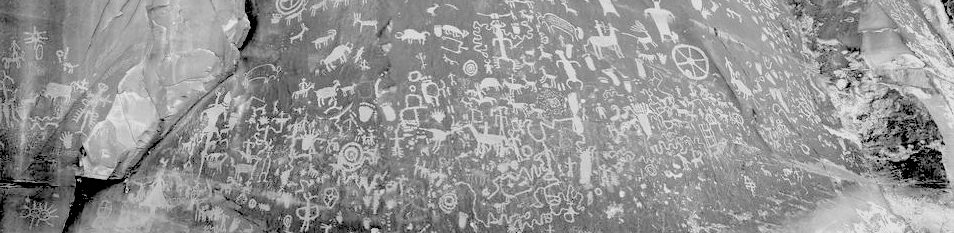
\includegraphics[width=\textwidth]{figures_c1/newspaperrock.jpg}
        \caption{\textbf{An example pictograph:} a 2000 year old petroglyth in Utah titled `Tse Hane' (rock that tells a story). Source:
        \citep{newspaperrock} }
        \label{cave}
\end{figure}


%
%
%
%


\subsection{The Origin Of Big Data}
The term `Big Data' originated in the mid-1990s, appearing in several job adverts and a slide deck by Jon Mashey, the chief scientist at Silicon Graphics (SGI), \citep{slidedeck,bigdataorigin}. This term is used as a way to describe the ever-increasing amount of data we can generate each day. Such phenomenons are seen in anything from the growing number of websites to the number of reactions within an explicit gas-phase chemistry mechanism, \autoref{fig:webmcm}. Coupled with the ability to collect large amounts of data is our requirement to analyse and understand it. This has commonly be done through the use of visualisation, a topic in which careful consideration must be made to ensure the correct information is conveyed \citep{kirk}. In a paper on mining big data, \citep{bigdatamine} explains that the main task of Big Data analysis is on deciding how to visualise the results- simply its size introduces complexity in uncovering a user-friendly method to represent the information required.

Although graphical representation has been an integral part of the data comprehension process, it is only relatively recently (1990's) that it is recognised as a research field \citep{ch6}. Even though we are not explicitly dealing with `big' data, the number of species and reactions occurring within the troposphere is still sufficiently large and complex that many of the same problems still exist. It is for this reason that this section\footnote{and consequently much of this thesis} we will explore the considerations that need to be made before selecting a visualisation design (\autoref{sec:visdes}) and the methods we can use to represent the complex relationships within the atmospheric chemistry domain (\autoref{sec:visrel}).

\begin{figure}[H]
     \centering
         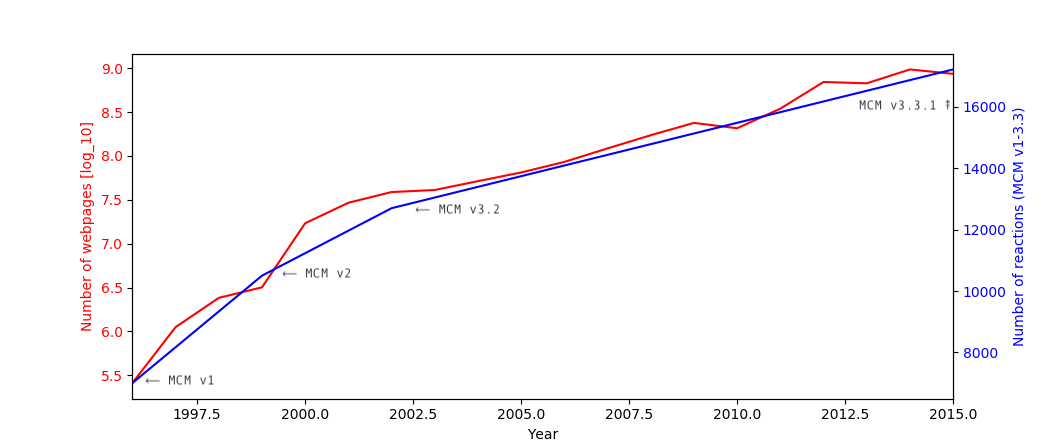
\includegraphics[width=.95\textwidth]{figures_c1/webmcm.png}
         \caption{\textbf{Data size and complexity increases with time due to (availability or improvements in scientific understanding).} The red line shows the change in the number of websites ($\log_{10}$ normalised) within the world wide web domain for years 1996-2015. Similarly, we compare the various releases of the master chemical mechanism (a discrete process), where more and more complex reaction schemes are iteratively appended over time. These are introduced later on. \\
 \emph{NOTE: The two lines are here to illustrate the growing trends between the subjects and are not incomparable due to their different scales and continuous/discrete natures.}\\ Source: \citep{webstats,mcmhist}}
         \label{fig:webmcm}
\end{figure}


\section{Visualisation Design}\label{sec:visdes}

New ideas are developed and refined through an iterative process of cognition and discussion with other researchers \citep{ch7}. As individuals, we are constrained by our experience and knowledge; novel ideas often consist of an amalgamation of many existing concepts \citep{wingedhorse,goodideas}. \citep{shapinginfo} explains that the process of understanding a visualisation depends heavily on the interaction between the user's internal knowledge and the ideas depicted within a visualisation.
This means that the careful selection of content and medium (of presentation) can directly influence what a reader takes away from the graphic. In its design, a visualisation must be both relatable (in metaphor) and intuitive (or explained through the use of storytelling).

%



\subsection{Storytelling}\label{sec:storytelling}

Storytelling is commonly used to highlight the process of cause and effect. It has applications in the education for both the explanation of scientific concepts (\citep{marsstory}) and the dangers of the world (fables such as Little Red Riding Hood and Goldilocks teach the dangers of speaking to strangers and the importance of respecting personal property). As human life is subject to the conditions of the `arrow of time', the inherent familiarity of linearly consequential events make the narrative a great way to inform the reader of new (unseen) concepts. Such methods are not limited to the education of young children, but also allow for the understanding of real-world events through the use of dreams, media and the news \citep{storyanimal,dream}.

In entwining narrative and visualisation, it is possible to provide the user with a higher level of understanding and enable them to draw their own (guided) conclusions from the data. \cite{eyestory} explains that within the visual analysis of a graph, users often create a narrative through the use of visual routine. Here emphasis is placed on storytelling to `guide' and educate the reader of any events which led to a conclusion - this uses a question-answer cause-effect structure. It is this process that makes `storytelling' an effective method of communication to a non-expert audience \citep{nonscientific}.


\subsection{Metaphor Selection}\label{sec:metaphor}
Storytelling often involves metaphors to create content which is relatable and intuitive to the user. Such metaphors have infiltrated many parts of our everyday lives ranging from descriptions in fables to the concept of money and belief that govern everyday life through the inter-subjective\footnote{The inter-subjective is something that exists within the communication network. It allows a fictional idea, such as a limited-liability company, to exist as a real physical entity with a bank account and subject to laws. } \citep{sapiens}. In general there exist three categories of metaphors which may be used - natural (\autoref{sec:metnat}), man-made (\autoref{sec:metman}) and composite (\autoref{sec:metcom}).

\subsubsection{Nature-Inspired}\label{sec:metnat}

Inspiration for metaphors often comes from objects or events encountered from everyday life - the most effective of which have an inherent familiarity for all readers. As nature is universal to everyone on the planet, a nature-inspired metaphor not only guarantees a basic level of item comprehension but also contain an aesthetically pleasing familiarity to them. Common examples of these can include the use of ice to represent glacial melting or trees to show branches in decisions (decision tree: \autoref{fig:1tree}) or temporal changes in conditions with a trunk cross-section style plot (\autoref{fig:trunk}). Natural metaphors are often useful in conveying complex ideas due to their low learning curve.

\begin{figure}[H]
     \centering
     \begin{subfigure}[b]{0.495\textwidth}
         \centering
         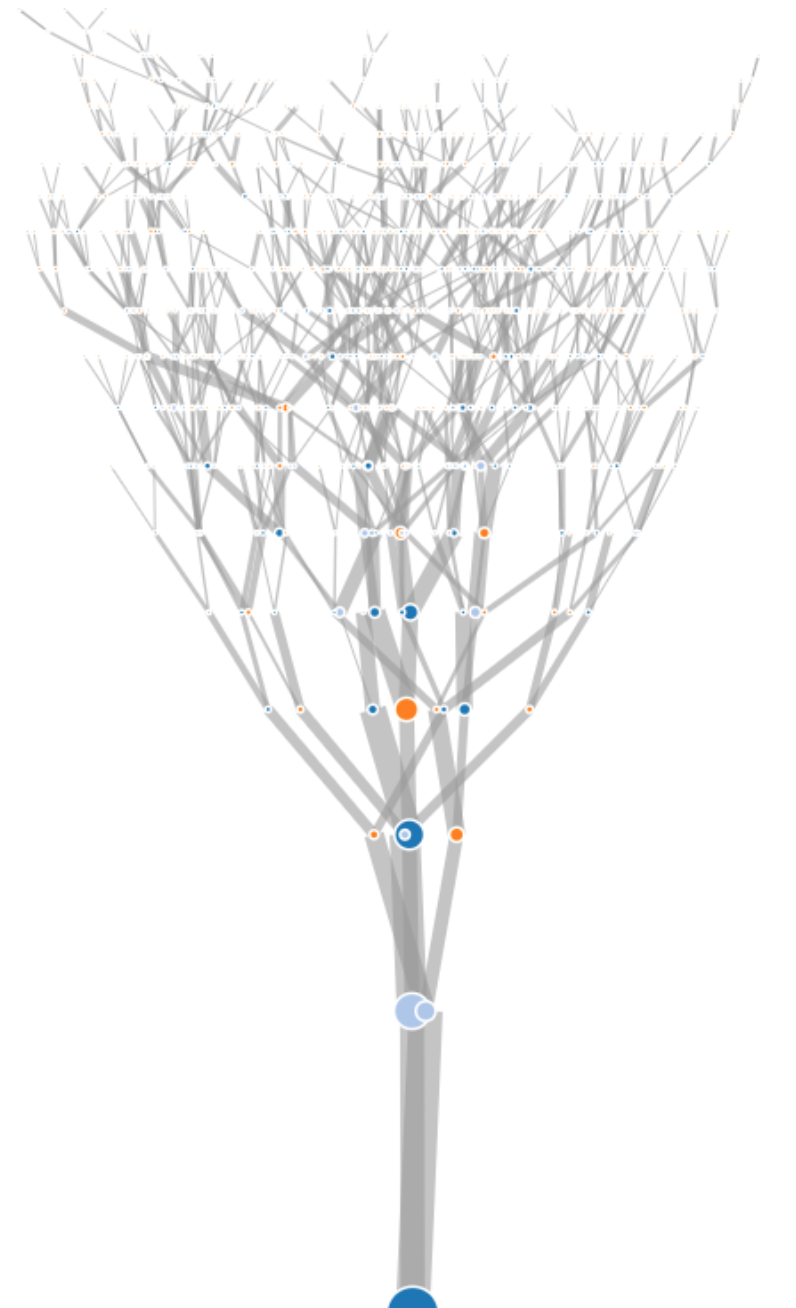
\includegraphics[width=0.8\textwidth,height=\textwidth]{figures_c1/tree.png}
         \caption{Single Tree (coloured leaves)}
         \label{fig:1tree}
     \end{subfigure}
     \hfill
     \begin{subfigure}[b]{0.495\textwidth}
         \centering
         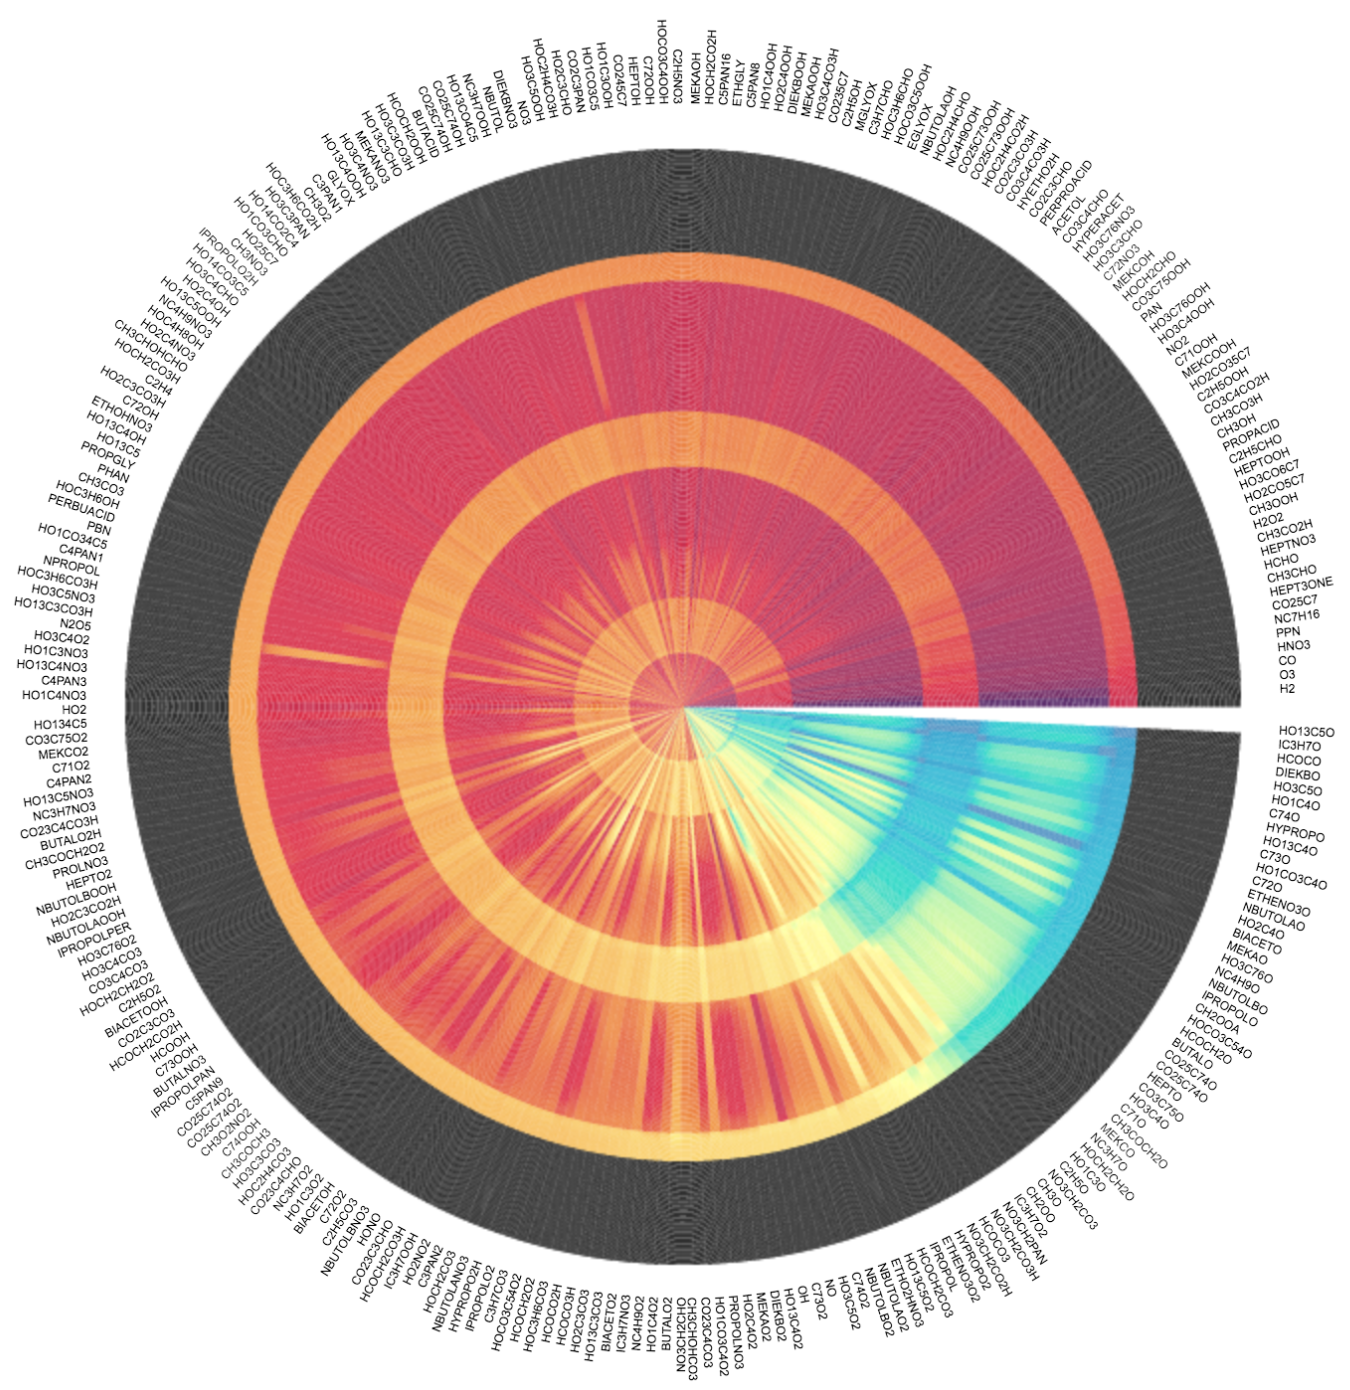
\includegraphics[width=\textwidth]{figures_c1/trunk.png}
         \caption{Complete tree trunk}
         \label{fig:trunk}
     \end{subfigure}


        \caption{\textbf{Two tree-inspired visualisations. }\\
         (a) shows the decisions made on a single decision tree within a random Forrest. Hear each branch split corresponds to a decision and the node/leaf colour represents the category of the decision. Stronger and more important decisions correspond to larger leaves and thicker branches. \\
          (b) shows a radial plot in the shape of a tree trunk. Here time is shown radiating outwards from the centre. This allows us to spot any changes in events - much like the rings of a tree can be used to identify when natural disasters (such as tsunamis or avalanches) have struck them. This specific visualisation shows the net flux of species from a chemical simulation.
These are coloured from low fluxes (blue) to high fluxes (red). The abrupt changes here show the diurnal cycle where photochemical reactions stop and then start up again. }
        \label{fig:trees}
\end{figure}


\subsubsection{Man-Made}\label{sec:metman}
Similar to nature, another similarity between many readers would be their familiarity with the urban environment. Metaphor inspiration from human-made objects such as buildings often contain characteristics of symmetry and manual/mechanical design. These allow the user to interpret any features presented using their pre-existing knowledge about an object. The most famous example of this is (\autoref{fig:beck}), where stations are positioned at 0,90 and 45-degree angles. This provides a clearer representation, much like a road map than the current space-specific location of each station. Although other designs, such as a concentric one, \citep{circ}, have been attempted, adaptations of Beck's design are still being used in the present day owing to their intuitive nature.


\begin{figure}[H]
     \centering
         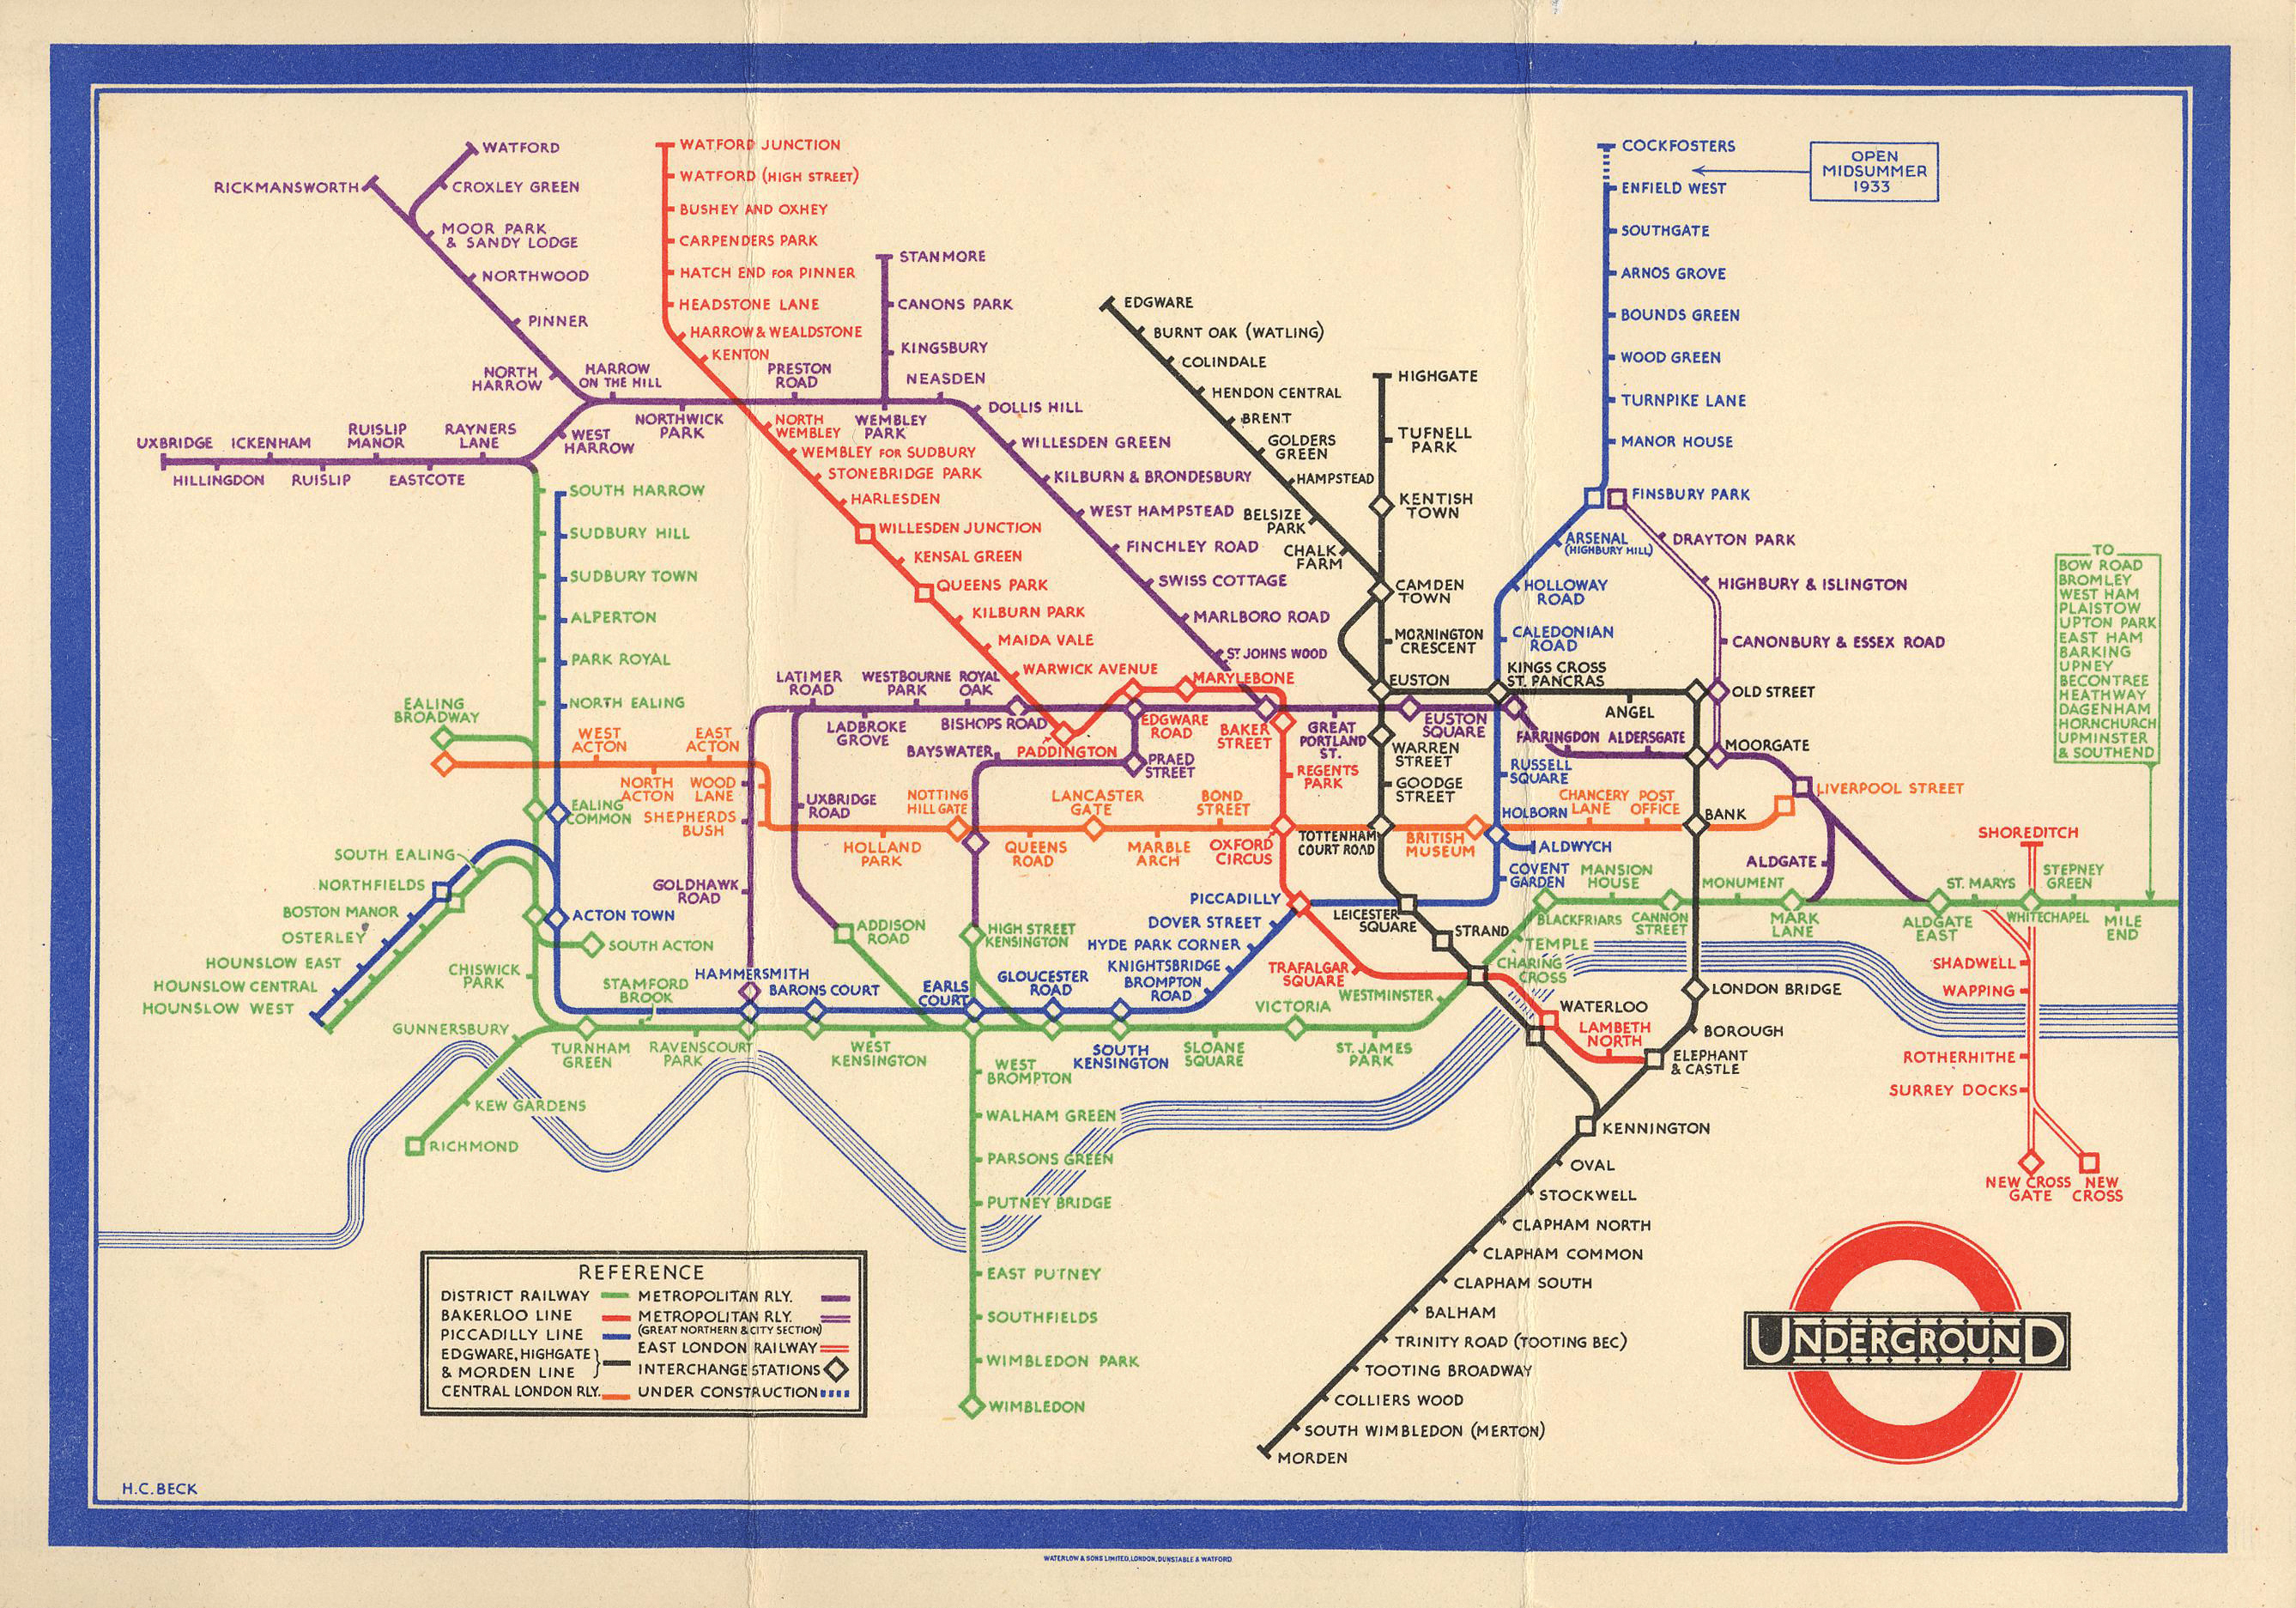
\includegraphics[width=.795\textwidth]{figures_c1/Beck_Map_1933.jpeg}
         \vspace{5mm}

         \caption{\textbf{The 1933 tube map design for London.} Source: \citep{beck}}

         \label{fig:beck}

\end{figure}

\subsubsection{Composite}\label{sec:metcom}

Finally, it is possible to combine ideas into a composite metaphor, a concept common in much of greek mythology. An example of this is Pegasus, where the combination of two familiar items (wings and a horse) results in something novel and unseen (a winged horse) which has implications from its existence associated with it.
Overcoming the problems presented by these composite designs involves a level of lateral thinking, prototyping (sketching) and redefining to produce a confluent user-visual metaphor interaction \citep{shapinginfo,fds}.

The development of new items can also be applied to the creation of xenographics -  here the combination of visualisations allows for the representation of complex relationships with a smaller learning curve. An example of this is the amalgamation of a  `pizza/pie chart'\footnote{There is a good amount of literature that suggests these are far from optimal methods of representing data. } with a bar chart to create a radial plot in \autoref{fig:nightingale} - A novel representation style which helped explain and establish the methods of modern-day nursing by Florence Nightingale.



\begin{figure}[H]
     \centering
         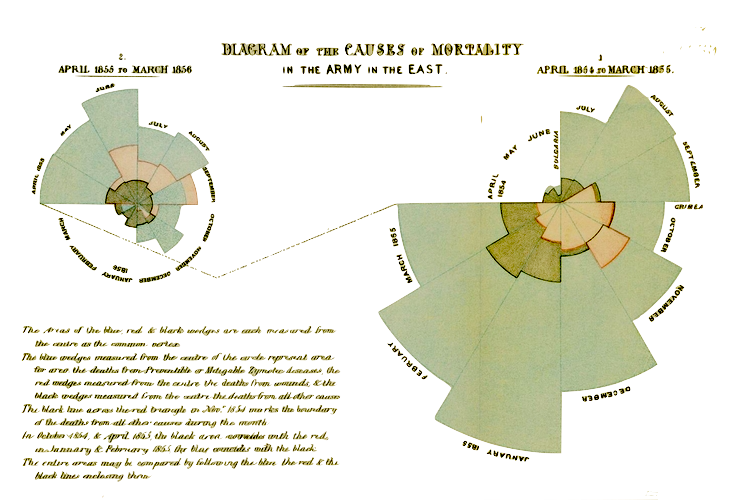
\includegraphics[width=.8\textwidth]{figures_c1/nightingale.png}
        \caption[Caption for LOF]{\textbf{A (stacked) Radial bar-chart showing the causes of mortality in the British army}\protect\footnotemark , \citep{nightingale}.}
        \label{fig:nightingale}
\end{figure}
\footnotetext{Also known as the Nightingale Rose or Coxcomb plot.}




\subsubsection{Domain Specific}




Composite designs are not constrained to the combination of different metaphors. In specialised roles, it is common to find visualisations which draw on pre-existing knowledge either about the content of the figure. Although this involves a new learning curve before information about the topic can be extracted, once this is obtained, the wealth and complexity that is portrayed by a single visualisation drastically increases. Two of the more common examples where prior knowledge is required to read a plot are connected plots\footnote{ Occasionally known as snail trail chart (R users seem to like re-inventing the wheel). } and Tephigrams.

\textbf{T-$\phi$-grams (Tephigrams)} are defined from their axis of temperature ($T$), entropy($\phi$) are used in the field of meteorology and weather forecasting. The combine grid lines for constant temperature (isothermic) and pressure (isobaric), as well as allowing the user to calculate the equivalent potential temperature for saturated air parcels and the saturation mixing ratio concerning plane water surface, \autoref{fig:tefidesc}. This provides a good example where both scientific knowledge and ability to read the diagram are required to obtain meaningful information from it.

\begin{figure}[H]
     \centering
     \begin{subfigure}[b]{0.4\textwidth}
         \centering
         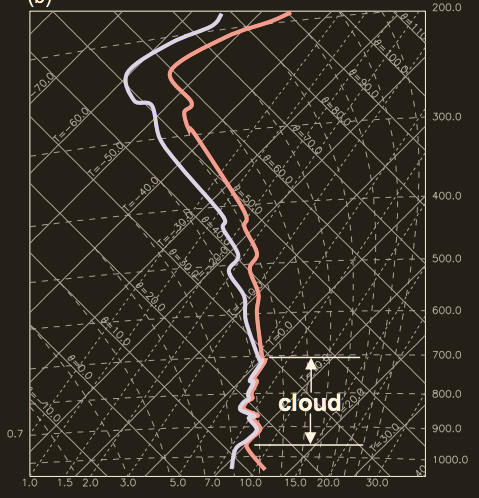
\includegraphics[height=1.325\textwidth,width=\textwidth]{figures_c1/tephiuse.png}
         \caption{A tephi diagram}
         \label{fig:tephidiag}
     \end{subfigure}
     \hfill
     \begin{subfigure}[b]{0.59\textwidth}
         \centering
         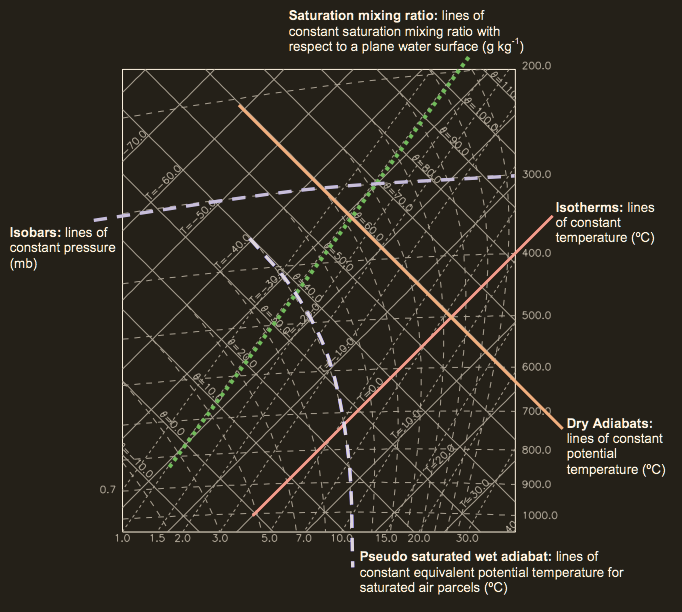
\includegraphics[width=\textwidth]{figures_c1/tephidescribe.png}
         \caption{Description of each axis on the tephi diagram. }
         \label{fig:tefidesc}
     \end{subfigure}
        \caption{\textbf{Two T-$\phi$-gram plots.} An example of the T-$\phi$-gram data (a),  and instructions on how to interperate it (b). The full scale figures are found within the source. Source: \citep{tephi}}
        \label{fig:tephi}
\end{figure}


\textbf{Connected scatter-plots} are useful in representing the temporal changes of correlation between to items. These are particularly useful in the field of economics due to their ability to highlight the different trends that can occur over time. \autoref{fig:conscat} shows how the number of vehicle-related fatalities changes with the number miles driven. In this situation, a simple $x-y$ plot may highlight a decreasing inverse relationship between the number of fatalities and the miles driven per capita over time, but lose some of the many features presented by the additional dimension.
\autoref{fig:conscat} b is an extract from \citep{defconscat}, which shows how the changes between two variables (blue and green) over time are represented within the connected scatterplot (yellow). Examples include unchanging variables (\autoref{fig:conscat}b.A) which are represented as a single point. Like correlations are shown by a 45 degree angle line (\autoref{fig:conscat}b.C) and inverse correlations are shown by a like orthogonal to the like concentration one (-45 degree)- (\autoref{fig:conscat}b.D).


\begin{figure}[H]
     \centering
         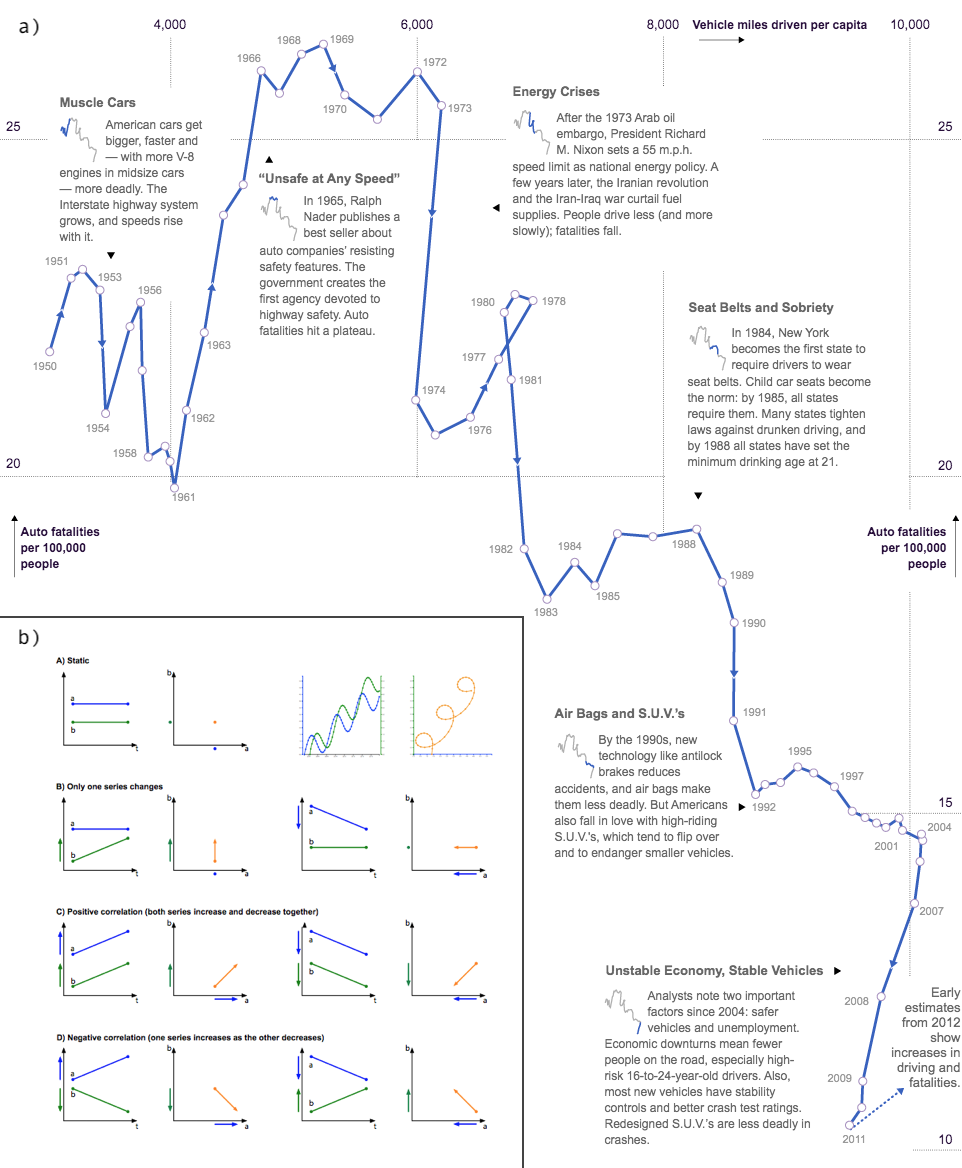
\includegraphics[width=1.1\textwidth]{figures_c1/connectedscatter.png}
        \caption{\textbf{Examples of connected scatterplots} (a) A connected scatterplot comparing the number of vehicle-related fatalities with the number miles driven per capita \citep{conscat}\\
        (b) a plot showing how the correlation of two spatial variables are transformed from a classical scatter/line plot into a connected scatterplot \citep{defconscat}. Here the blue and green lines represent different values changing over time (orange) across the x-axis. The figures to the right show how different correlations are transformed into a connected scatter plot, where the variables (blue and green) are plotted across each axis, and time (orange) is shown as a line joining each datapoint. The data points are plotted in equal lengths of time, meaning that the distance between consecutive points informs us of the amount each variable has changed.}
        \label{fig:conscat}
\end{figure}
\newpage




\section{Visualising Relationships}\label{sec:visrel}

Visualisation is important in conveying the impact of science and data to both the expert (e.g. complex figures in \citep{IPCC2007Science}) and non-expert (gross over-simplifications, e.g. the climate stripes \citep{stripes}). This section builds on the considerations discussed in the previous chapter and explores the different ways in which the relationship between species in the troposphere can be represented. We start by defining the dataset (\autoref{sec:dataset}) and then discuss several different visualisation methods (\autoref{sec:sociographs}).

\subsection{The Dataset}\label{sec:dataset}

Within an atmospheric chemical model, the chemistry of the troposphere is described using a chemical mechanism. The chemical mechanism used in this thesis is known as \emph{the Master Chemical Mechanism} (MCM) v3.3.1, which contains  5809 species and 17224 reactions \citep{mcm}. The MCM is a near explicit representation of our understanding of the gas-phase chemistry within the troposphere. In its mathematical form, it describes how species are related and at what rate they react.



 As the aim of this section is to identify essential features within the chemical mechanism we begin by looking at the mechanisms construction protocol (\autoref{fig:mcmprotocol} and [\autoref{fig:protocol} which is the protocol for MCMGecko, but is highly similar to that of the main MCM and provides a better representation of the computational decisions used in mechanism construction]). This construction methodology mimics the reasoning and procedures performed by an analytic chemist and allows for the simultaneous construction of a consistent and compatible chemical mechanism between several areas of research.  The procedure is becoming semi-automated and follows several iterations starting from a set of primary emitted VOCs. These are run from the protocol to build a set of degradation reactions in which the selected species may undergo. Any new products are then introduced to the procedure until everything has been oxidised to produced carbon dioxide and water. This produces the set of near explicit equations which are then used to describe the evolution of chemistry within an atmospheric model.

\begin{figure}[H]
     \centering
         \centering
         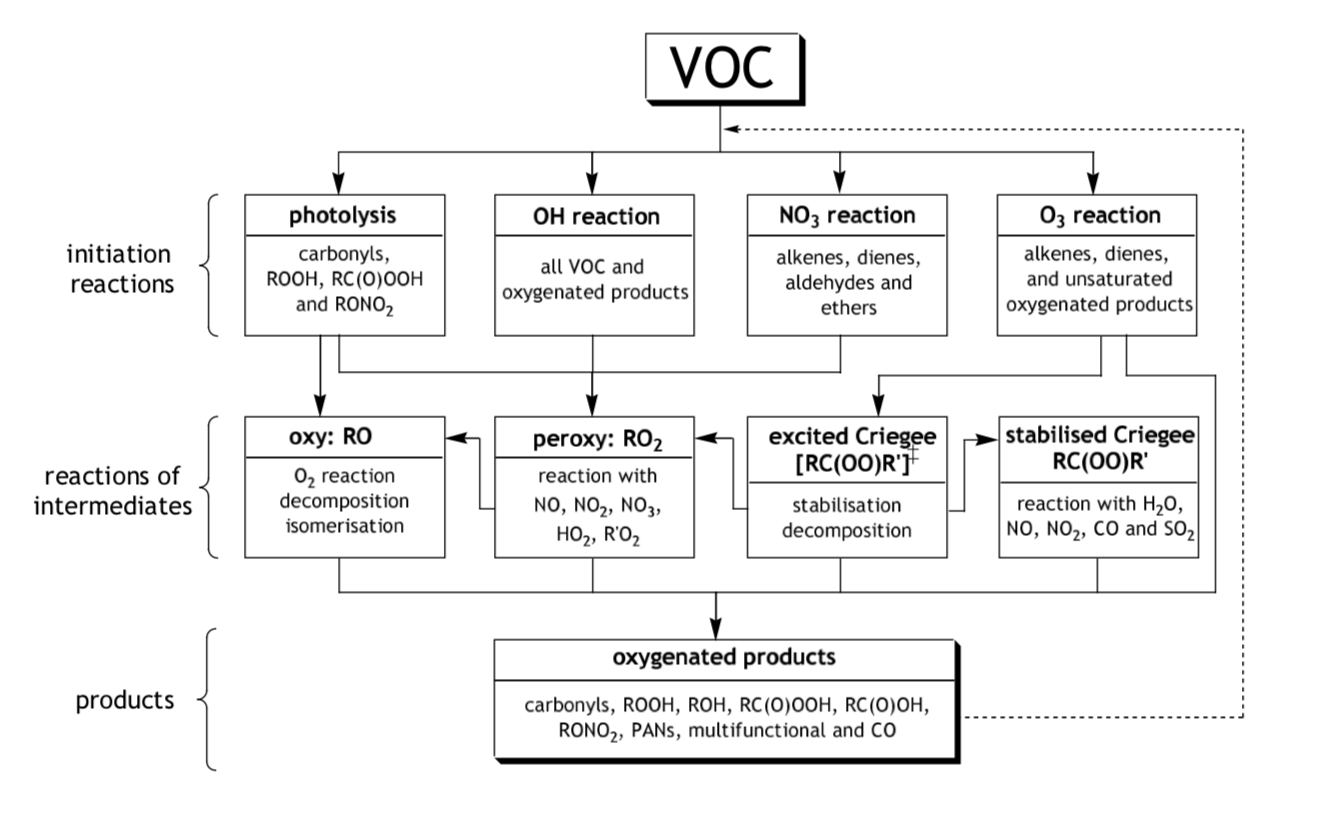
\includegraphics[width=.96\textwidth]{mcmproto.png}
         \caption{\textbf{The generation flowchart used within the MCM.} This shows the process undergone by a new species to generate its products. Any unseen products are then fed back into the flowchart until the entire mechanism has been produced.  Source:\citep{mcmpartA}}
         \label{fig:mcmprotocol}
     \end{figure}


     \begin{figure}[]
          \centering
              \centering
              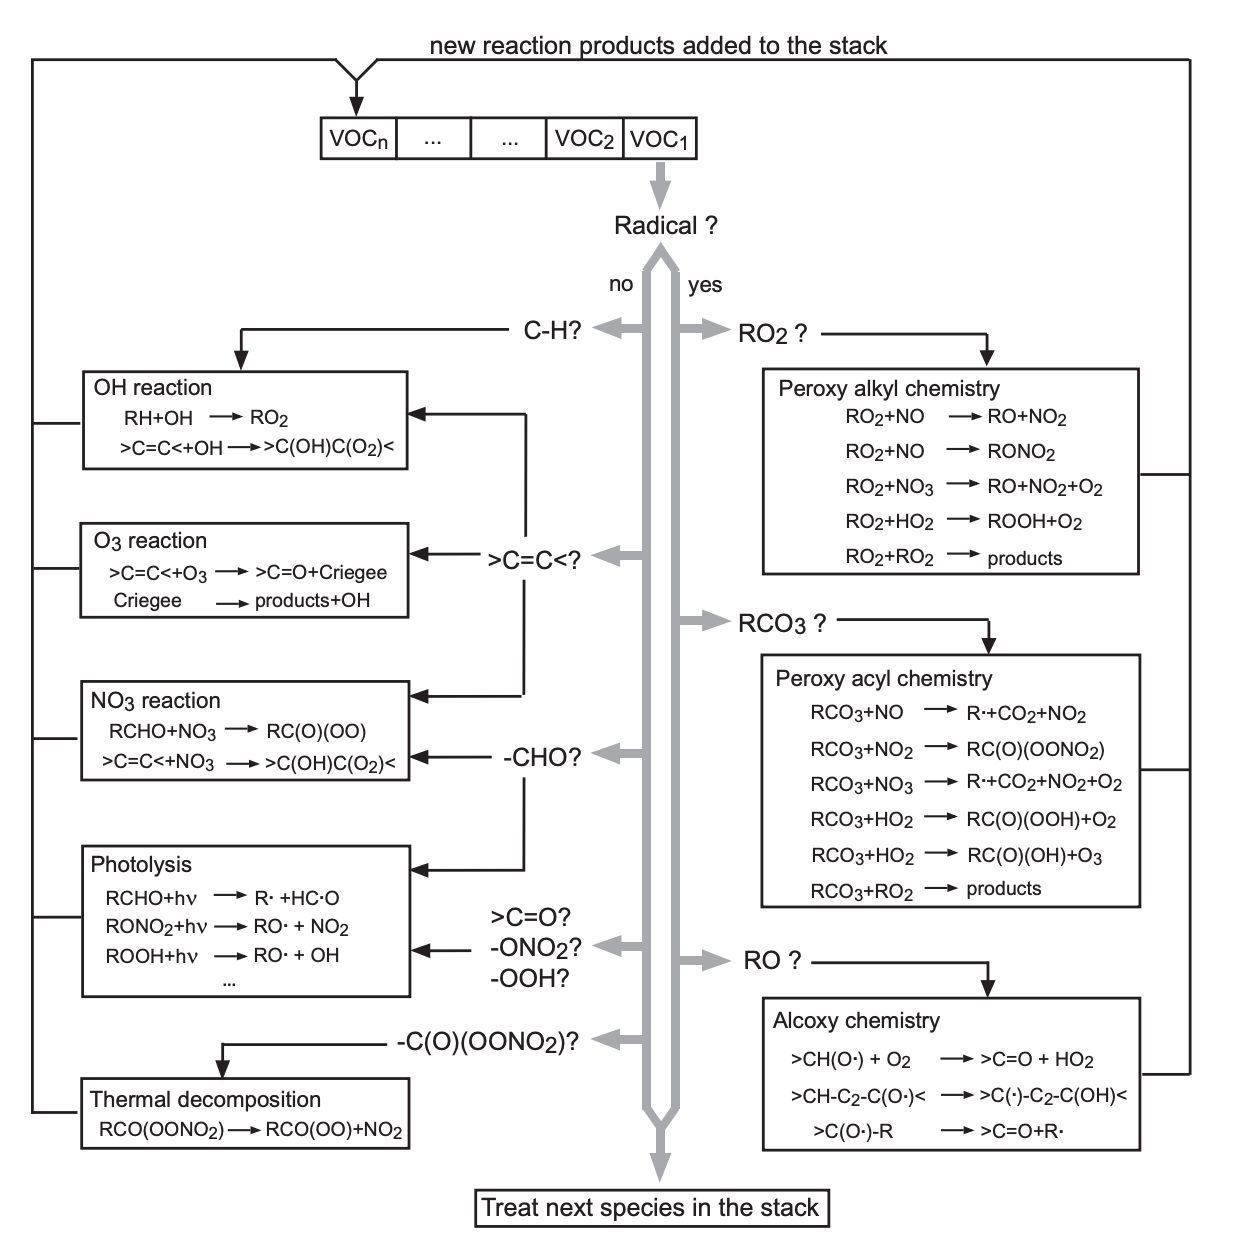
\includegraphics[width=.96\textwidth]{figures_c1/generation.png}
              \caption{\textbf{The generation flowchart used within Gecko.} This is very similar to the MCM protocol (\autoref{fig:mcmprotocol}), but provides a clearer representation of the machine read desicions for the mechanism generation.  Source:\citep{protocol}}
              \label{fig:protocol}
          \end{figure}

\subsection{The Sociograph}\label{sec:sociographs}
Social network analysis is a type of sociological work (sociometry) that aims to reveal the interweaving and interlocking relations between items or individuals, \citep{socialorigin}. \citep{gossip} argues that the evolution of language as a result of social grooming (gossip), and therefore its adaption for storytelling. It follows that using the social network construct to represent the underlying patterns between objects makes use of both our inherent ability to discern complex patterns through the use of storytelling. In trying to depict the relationships between a social network, we employ the use of sociograms. These are a class of visualisations which reveal certain properties of a social network. The following section will look at the extraction of useful information from the relationships within the MCM through the use of several sociograms.

\subsubsection{The Chord Diagram}
A chord diagram is a visual sociogram known for its use in summarising the overarching relations within a dense social network \citep{chord}. Here arcs are used to represent groups (or a node from a social network graph), and their length corresponds to the percentage of items they contain. Within \autoref{fig:chord} we represent the different routes a species may react within the MCM protocol flowchart shown in \autoref{fig:protocol}. The figure contains two sets of arcs. These represent the different level of classification of the chemistry - The first (outer) arc represents the split in channels between radical (red) and non-radical (orange) species which further separated into the finer categories within each branch (the labelled inner arcs). The inner arcs again show the probability a randomly chosen reaction on a species will fall under a particular category - if we convert an arc into a segment we have a pie chart of probability.

\textit{It is worth noting that segment sizes do not represent the number of species undergoing a specific reaction pathway, but rather the percentage of all possible pathways which follow that route. This is because species often undergo a range of reactions, each of which counts as an individual weighting. It is for this reason that even though almost all\footnote{ Except for any inorganic species.} contain a C-H bond, hydrogen abstraction does not consume the whole graph. Many species have multiple possible pathways in which they may react, and the chord diagram presents the likeliness of a rection for all possible methods of reaction for all species.
}

From this, we see that hydroxy reactions are the most common with C-H bonds being in abundance\footnote{This is seen within the graph layout \autoref{fig:mcmfull}}. We also see that having another type of reaction is also just as probable, with a third of the most utilised branches within the MCM protocol falling under species containing at least one Carbonyl group.
Next, we look at the co-occurrence of branches for different species. These are represented using the area of a circle connecting two arcs (a chord). Each chord has two edges connecting two arcs\footnote{ except for self-loops, although these are addressed below.}.  It is possible to discern the percentage of items going between these and other branches by comparing the width of each chord to its parent arc. Here, for example, we see a roughly even split between species with a C-H bond (i.e. all species) and every other group. This suggests an even distribution of reaction types between species.
This means that in comparing the arc length of each chord, we can visually determine the percentage of group A which relates to its partner group B. Finally it is also possible to determine the number of items in a group which contain themselves. Chemically these are species with multiples of one functional group that undergo a specific reaction pathway more than one time. Although these reactions will usually be combined within a mechanism (to avoid duplication), their rate would be increased accordingly.

\begin{figure}[H]
     \centering
     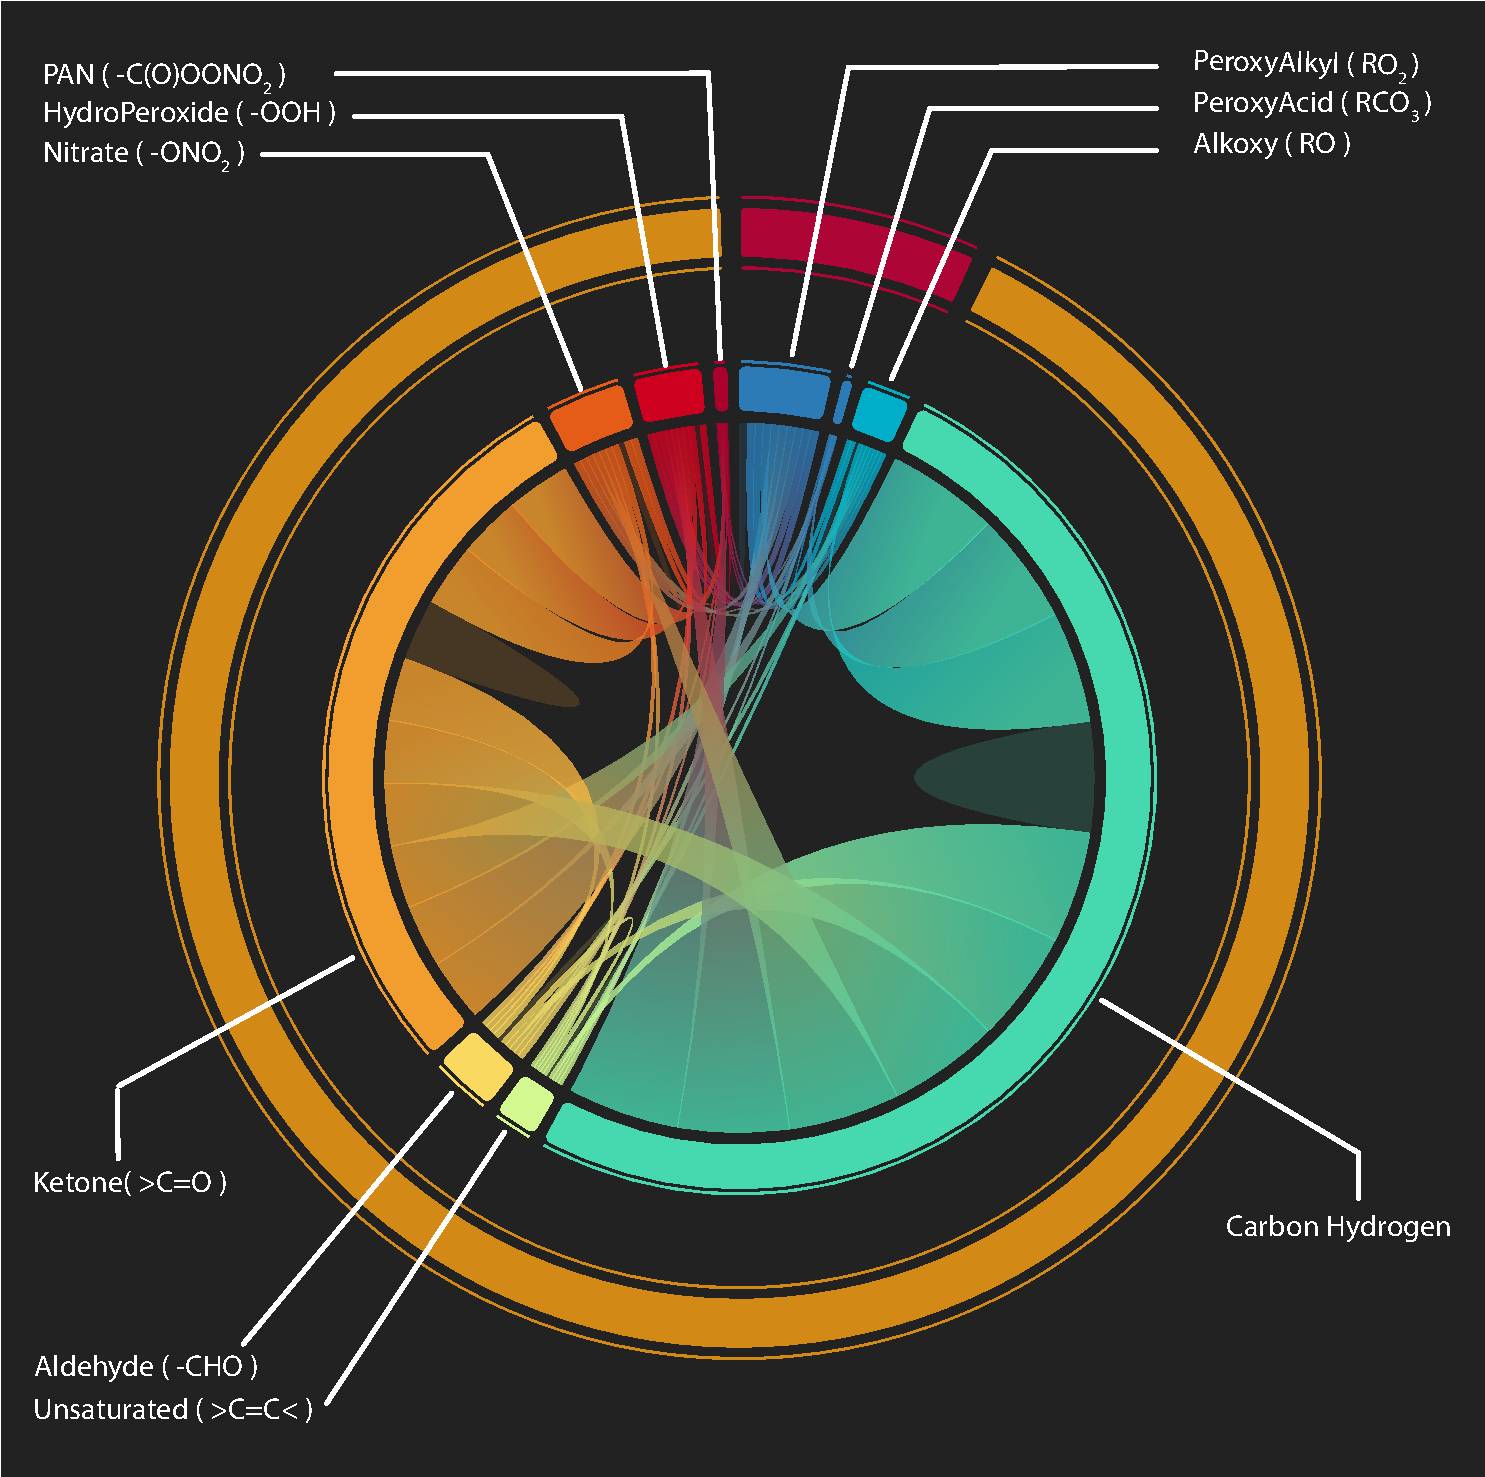
\includegraphics[width=\textwidth]{figures_c1/radicallayermcmgen.pdf}
        \caption{\textbf{A chord diagram of the protocol structure}. This shows the proportional probability a species from the MCM will follow one or more of the paths presented in \autoref{fig:protocol}. The outside ring represents the radical (red), and non-radical (gold) split between groups. The inside ring splits these into individual groups, providing a finer level of detail. }
        \label{fig:chord}
\end{figure}


The chord layout provides an easy way to calculate the percentage of items which contain multiple properties. It requires a relatively low learning curve and is intuitive to those with experience using pie charts (namely the Microsoft Office generation), however, this radial format can sometimes also make it more challenging to read. Special attention needs to be paid to the order arcs are drawn, as with some datasets, specific configurations may obfuscate trends. Finally, the chord diagram requires a certain amount of data munging before its employment. It is due to this that finer details about the system may be lost, especially if there is a course scale between chord sizes.



\subsubsection{Direct Representation Of The Relational Matrix}
Relational matrices, also known as the adjacency matrix, are a $n \times n$ square matrix highlighting the relationships between items. These can be constructed (or used to construct) a graph and provide the easy identification of patterns between nodes. \autoref{fig:adj} shows an MCM subset of propane sorted by the number of carbons. Here we see that for this limited sample species tend to have slightly more reactions with other species with the same number of carbons than with different numbers.


The main downside of visualising the adjacency matrix is the sparsity of many real-world graphs (\autoref{ch3}). If we take the complete MCM v3.3.1 network \citep{mcmpartA} and visualise it in this manner, it will have a density of $5.9 \time 10^{-4}$. This means that for an average $600 \times 600$ pixel figure, only $0.36^2$ of a pixel would be coloured in. Moreover, since we are not able to colour only parts of pixels, our final plot will remain blank. Methods to circumvent this involve looking at subgraphs, or individual sections interactively or applying composite graph/adjacency techniques such as those presented in NodeTrix, a method for visualising sparse small world networks\footnote{Small world networks are discussed in the following chapter.} \citep{nodetrix}
%



\begin{figure}[H]
     \centering
     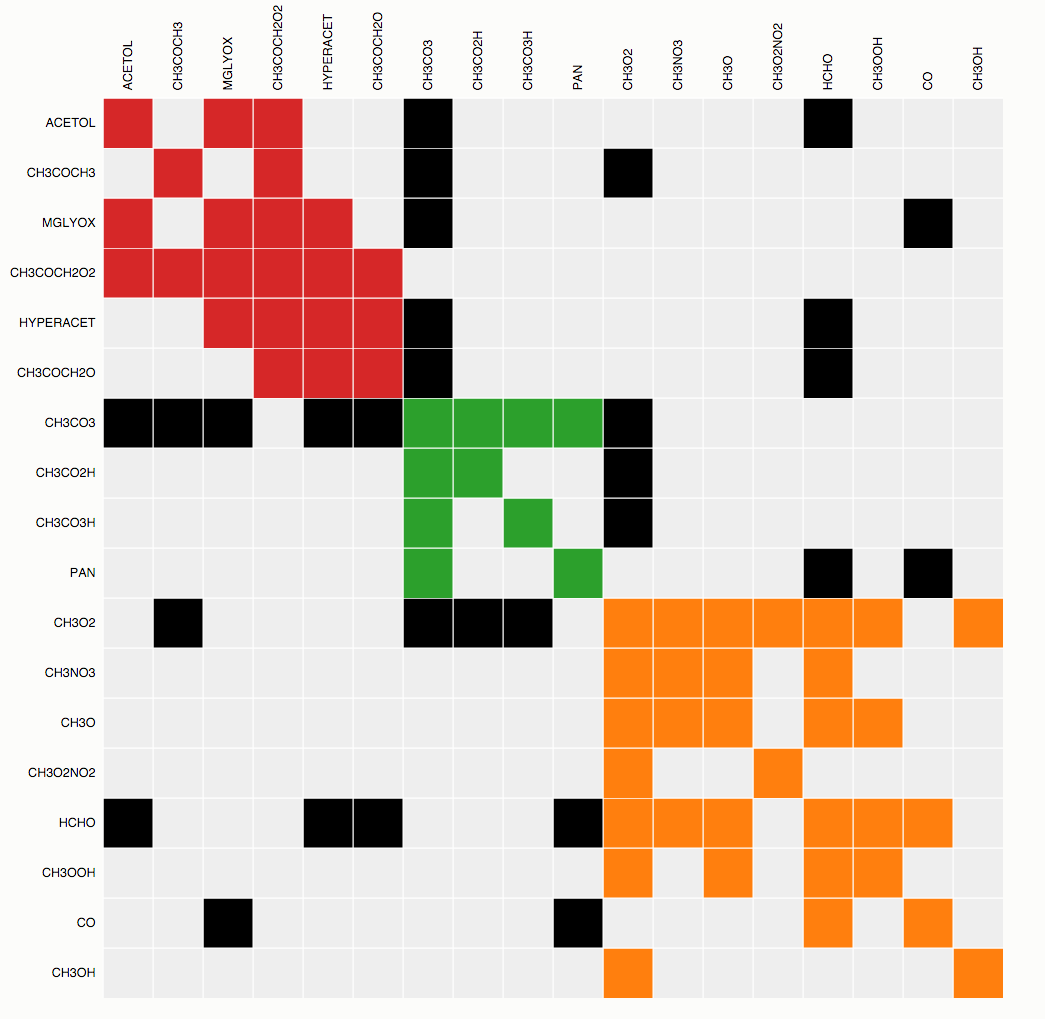
\includegraphics[width=.7\textwidth]{adjmatrix.png}
      \caption{\textbf{The adjacency or relational matrix is showing species from a propane subset of the MCM}. Here species are sorted by the number of carbons they contain (red$=3$, orange$=1$). Black cells represent reactions between species containing different numbers of carbons. If looking at clusters in a network (\autoref{ch4}) sorting elements in an adjacency matrix aid in the visual identification of these. Squares features along the diagonal indicate a larger number of links between grouped items colocated in the axis, and less to those in other locations (clusters).}
        \label{fig:adj}
\end{figure}

\subsubsection{Arc Diagrams}
Arc diagrams are a subset of sociographs where items are represented as nodes along the horizontal. Relationships between nodes are then shown through the use of curved links (arcs). It is this that makes them particularly suited for the highlighting of repetition between music or DNA sequences, \citep{arc}. Using the MCM database, we can construct an arc diagram to explore how species containing the same combination of functional groups react. This is done by first determining all branch permutations from the protocol flowchart (\autoref{fig:protocol}). This produces 179 groups which are positioned across the $x$ axis in ascending group size (the more branches matched, the further to the right a group is positioned).

\begin{figure}[H]
     \centering
     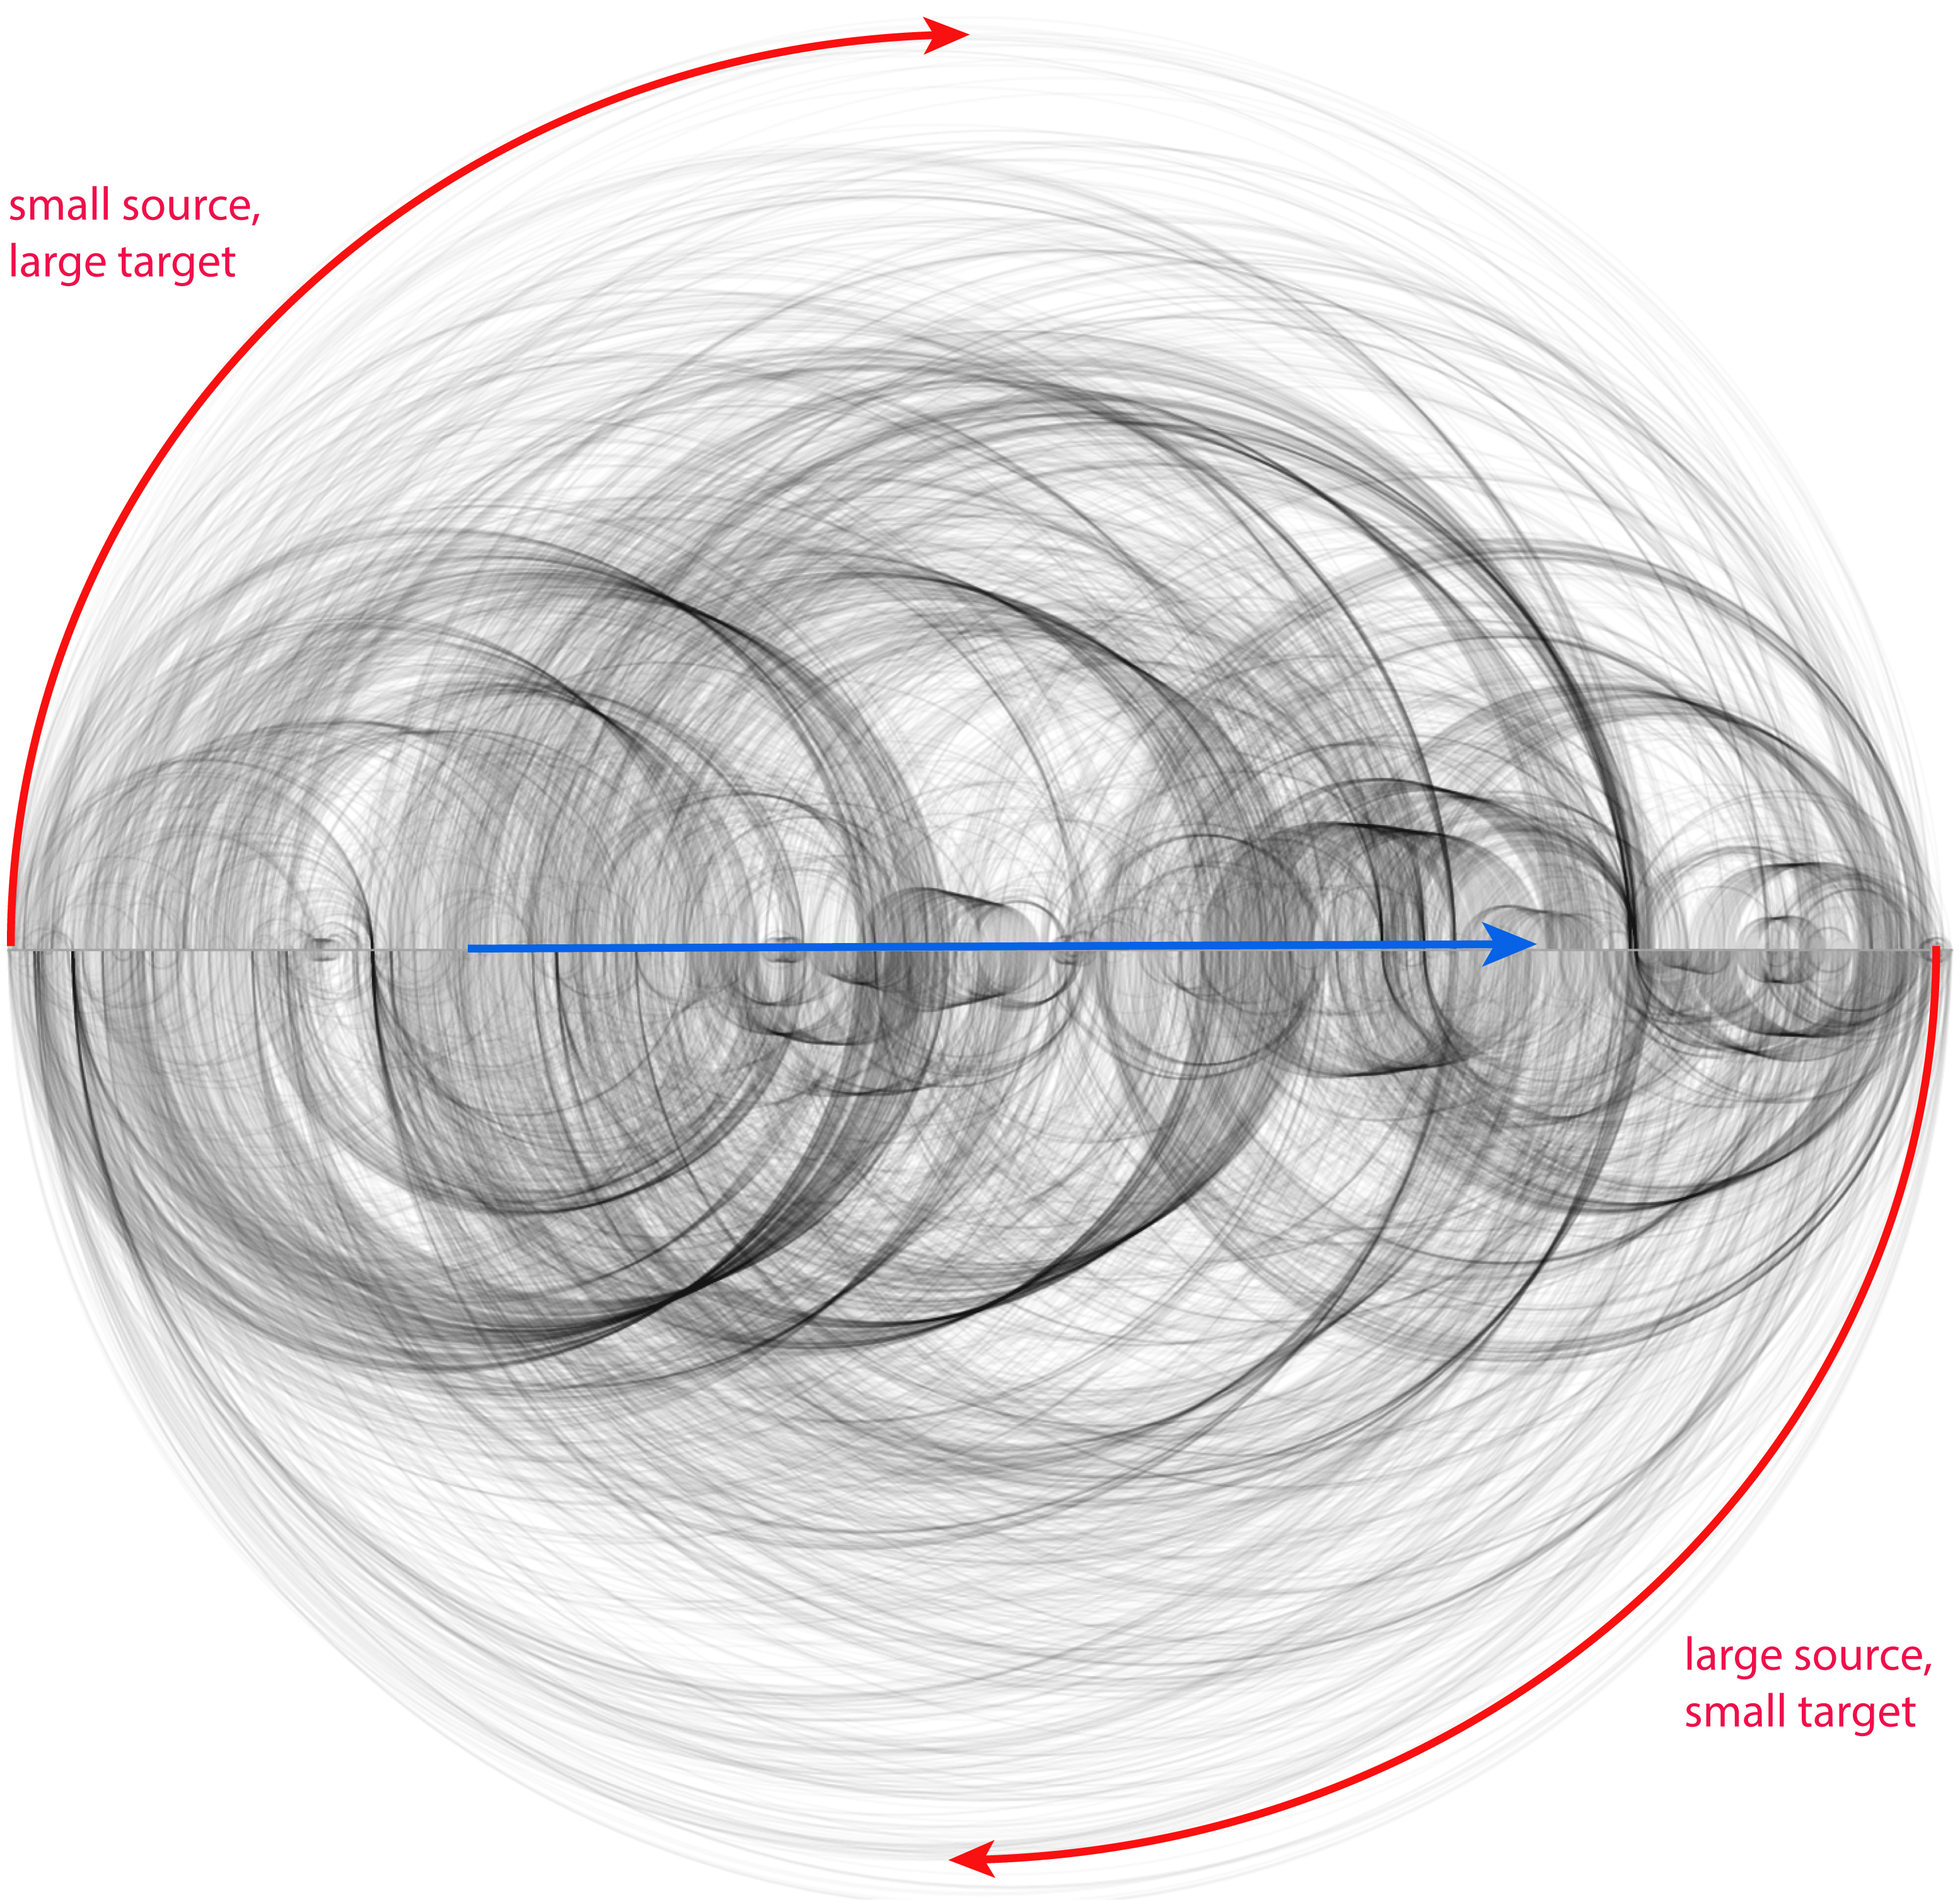
\includegraphics[width=.8\textwidth]{figures_c1/arc/arc_all.png}
     \caption{\textbf{An arc diagram from the MCM database derived by the protocol (\autoref{fig:protocol})}. All possible pathways for each species are extracted. These are then grouped and sorted by the number of functional group/pathways available. Species are shown along the blue line and sorted by increasing number groups to the right. Reaction pairs (reactant-product) are then depicted through the use of arcs. If a species reacts to produce a species with more functional groups, it is represented by a forwards facing arc. If the product contains a smaller number of functional groups, the drawn arc moves downwards and backwards.}
     \label{fig:arcdiagram}
\end{figure}

The width of each group is determined from the number of species within it. Following links are added between the species based on what groups the product species from each reaction contain. \autoref{fig:arcdiagram} discretises reactions which produce products with an increased number of reaction pathways (positive arcs - top), from those which result in species with less (positive arcs - below). Here the cyclic nature of tropospheric chemistry can be seen, with many species producing larger, less stable, products, which then go on to react and decompose back into smaller ones. In some cases, a complete circle between two nodes can be indicative of a catalytic reaction.  Using interaction and selective shading, it is possible to isolate specific types of reactions and determine which of the functional groups are responsible for the change experienced within a reaction.

Although such a layout may seem daunting at first, with many lines, in all directions, filtering by type of reactions can draw attention to several features from the chemistry. In \autoref{ch0}, the importance of $HO_x$ cycle for the removal of VOCs and greenhouse gasses was discussed. For this reason, we begin by using arc diagrams to explore the relationship between OH and \ce{HO2} (\autoref{fig:ho2oh}).

\autoref{fig:ho2} and \autoref{fig:oh} show arc diagrams where the reactions of interest (photolysis and OH reactions respectively) highlighted in both colour and opacity. These enable us to see patterns between the radical cylcing of \ce{OH -> HO2} chemistry (\autoref{fig:rxnho2oh}). Here the cyclic reaction shown between the dashed lines corresponds to the reaction of \ch{RO2 <->[HO2][O2] ROOH} (\autoref{fig:rxnho2oh}).

Applying the same methodology to photolysis and hydroxide reactions, the production of species containing fewer functional groups is seen in \autoref{fig:ohhv}. Within the highlighted reactions, it is seen that a ROOH species undergoes a reaction with OH or photolyses (\autoref{fig:rxnohhv}). In the OH reaction, Hydrogen abstraction is performed to produce an RO2 species and water, \ch{ROOH ->[OH] RO2 + H2O}. Photolysis reactions, however, photolyse the double bond, \ch{ROOH ->[hv] RO2 + HO2}, reducing the number of functional groups - producing a larger arc. It should be mentioned that the ROOH can also react with \ch{o2} to produce an RO2, although this has not been highlighted.

Finally, Peroxy Acetyl Nitrates (PANs), play a vital role in the modelling of photochemical smog (ozone events), \citep{pans}. PANs an effective reservoir species with significant importance within the production of ozone in atmospheric chemistry models (especially if transportation is involved) \citep{finlayson}. Although they are very stable at cold temperatures, these can quickly decompose (thermally) to release $NO_x$ if warmed. In the MCM the thermal decomposition of PANS is determined by the KBPAN rate constant. In comparing reactions of \autoref{fig:kbpans}, with those of \autoref{fig:no2} (at rate KFPAN), we see a cycle between two arcs forming (\autoref{fig:pandir}). This can be explained by the reactions in \autoref{fig:rxnpan} which show that \ch{RC(O)OONO2 ->[KBPAN]  RC(O)O2} (+\ch{NO2}) \ch{ ->[NO2] RC(O)OONO2}.

\textit{\textbf{NOTE:} A downside to the arc diagrams format that has been chosen is that for reactions between species of the same number of functional groups, there is no set direction. }



\begin{figure}[H]
     \centering
      \begin{subfigure}[b]{.4\textwidth}
         \centering
         \includegraphics[width=\textwidth]{figures_c1/arc/ho2oh.png}
         \caption{The most prominent branches. }
         \label{fig:ho2oh}
     \end{subfigure}
      \begin{subfigure}[b]{.4\textwidth}
         \centering
            \scalebox{.7}{
        \schemestart [0,1,thick]
            \chemfig{R-[:-30](=[:-90]O)(-[:30]O-[:-30]O_{.})}
             \arrow{->[\ce{HO2}][][][.5][]}
            \chemfig{R-[:-30](=[:-90]O)(-[:30]O-[:-30]OH)}
            \arrow{0}[,0] \chemfig{\+ \ce{O2}}
         \schemestop\par
     }\\ \ \\
    \scalebox{.7}{
        \schemestart [0,1,thick]
            \chemfig{R-[:-30](=[:-90]O)(-[:30]O-[:-30]OH)}
            \arrow{->[\ce{OH}][][][.5][]}
            \chemfig{R-[:-30](=[:-90]O)(-[:30]O-[:-30]O_{.})}
            \arrow{0}[,0] \chemfig{\+ \ce{H2O}}
         \schemestop\par
         }\hfill
         \caption{Reactions observed}
         \label{fig:rxnho2oh}
     \end{subfigure}
     \begin{subfigure}[b]{.4\textwidth}
         \centering
         \includegraphics[width=\textwidth]{figures_c1/arc/ho2.png}
         \caption{\ce{HydroPeroxy}}
         \label{fig:ho2}
     \end{subfigure}
     \begin{subfigure}[b]{.4\textwidth}
         \centering
         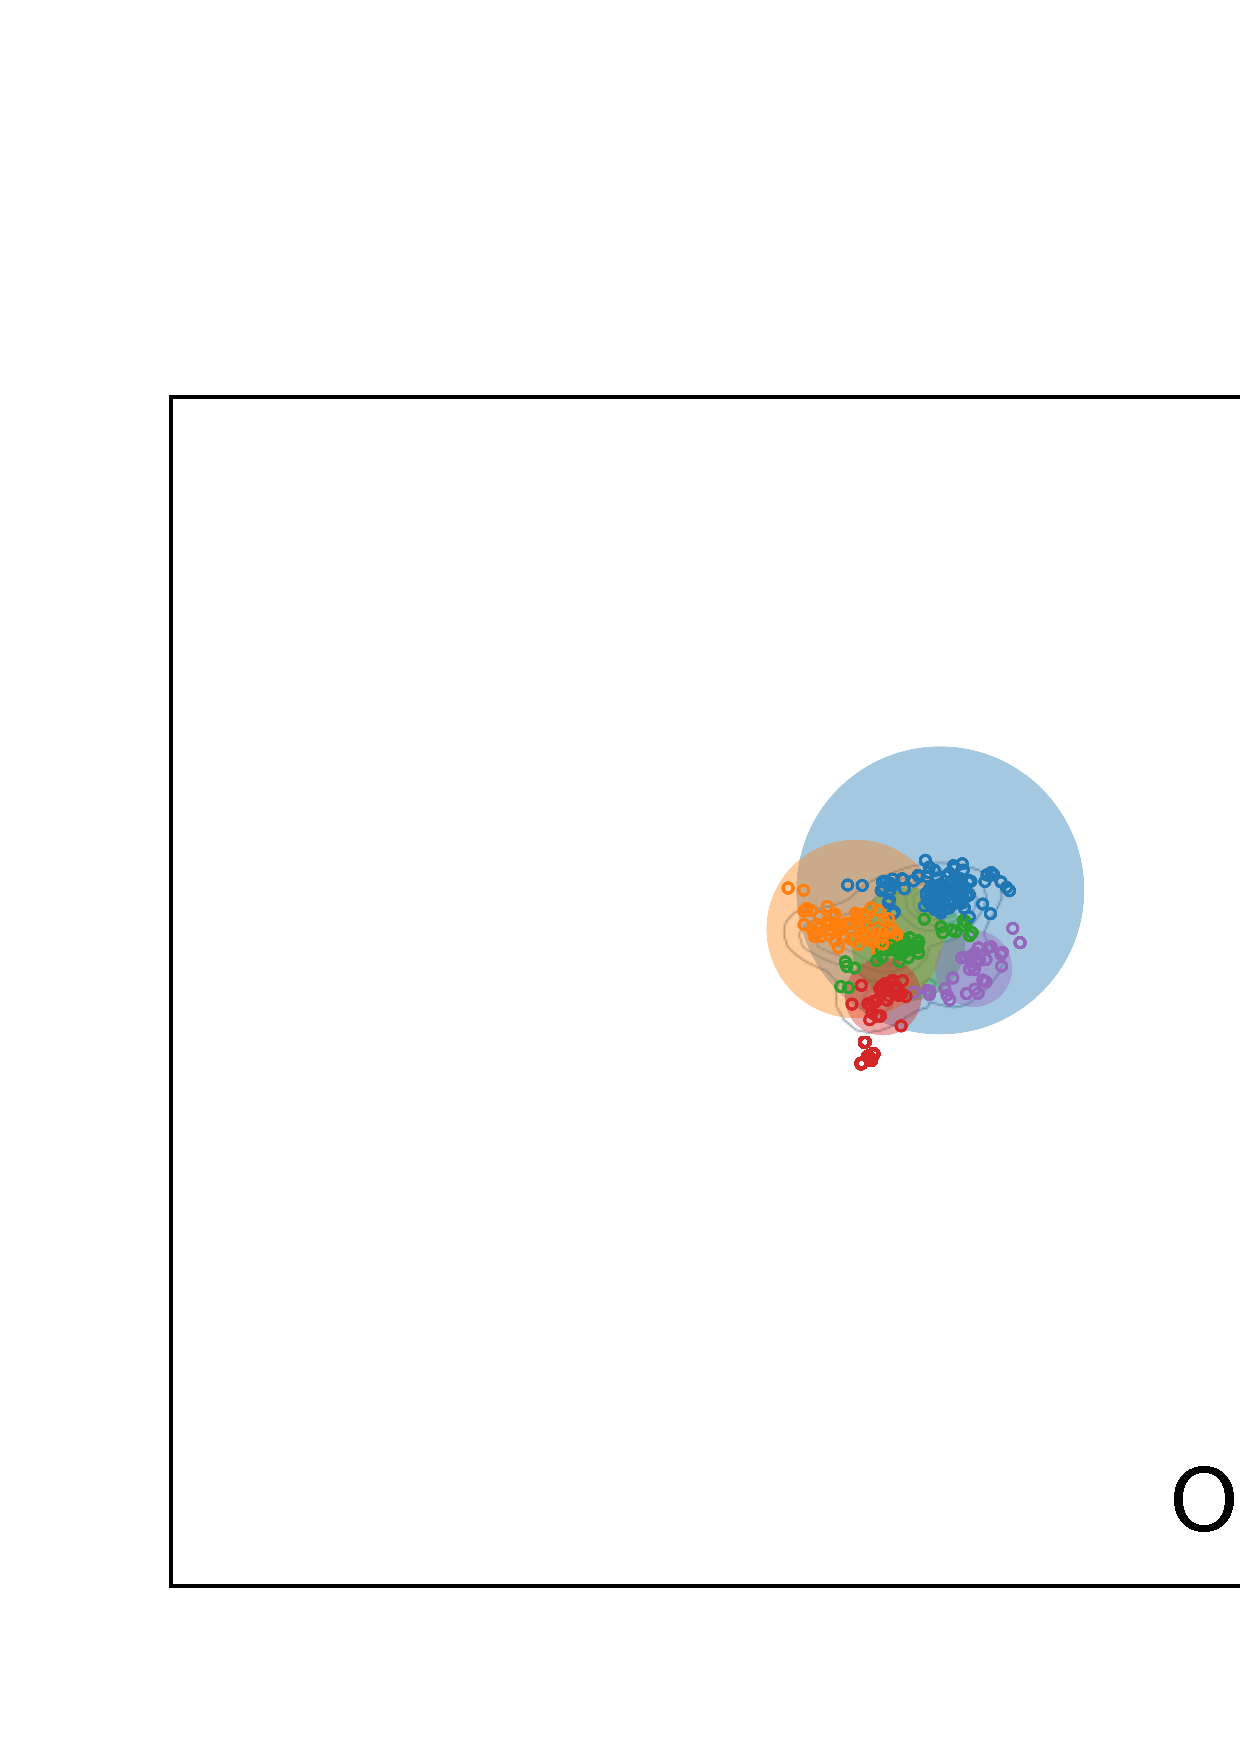
\includegraphics[width=\textwidth]{figures_c1/arc/OH.png}
         \caption{Hydroxide}
         \label{fig:oh}
     \end{subfigure}
      \caption{\textbf{ Arc diagram features for the Hydroperoxyl and Hydroxide radicals.} The $HO_x$ cycle chemistry (b) can ge seen within certain groups in the network. The main ones of these are hilighted in (a).   }
        \label{fig:ohho2}
\end{figure}



\begin{figure}[H]
     \centering
      \begin{subfigure}[b]{.4\textwidth}
         \centering
         \includegraphics[width=\textwidth]{figures_c1/arc/ohhv.png}
         \caption{The most prominent branches. }
         \label{fig:ohhv}
     \end{subfigure}
      \begin{subfigure}[b]{.4\textwidth}
         \centering
    \scalebox{.7}{
        \schemestart [0,1,thick]
            \subscheme{\chemfig{R-[:30](=[:90]O)-[:-30]O-[:30]OH} }
             \arrow(@c2--){->[$hv$]}[-25,1.8]
              \chemfig{R-[:30]O-[:-30]O_{.}}
              \arrow{0}[,0] \chemfig{\+ \ce{HO2}}
              \arrow(@c2--){->[OH]}[20,1.8]
              \chemfig{R-[:30](=[:90]O)-[:-30]O-[:30]O_{.}}
              \arrow{0}[,0] \chemfig{\+ \ce{H2O}}
         \schemestop\par
         }\hfill
         \caption{Reactions observed}
         \label{fig:rxnohhv}
     \end{subfigure}
     \\ \ \\
     \begin{subfigure}[b]{.4\textwidth}
         \centering
         \includegraphics[width=\textwidth]{figures_c1/arc/hv.png}
         \caption{$hv$}
         \label{fig:hv}
     \end{subfigure}
     \begin{subfigure}[b]{.4\textwidth}
         \centering
         \includegraphics[width=\textwidth]{figures_c1/arc/OH2.png}
         \caption{Hydroxide}
         \label{fig:oh2}
     \end{subfigure}
      \caption{\textbf{ Arc diagram features for photolysis and  hydroxide. reactions.  } Photolysis results in species with a reduced number of functional groups, and therefore longer arcs. OH reactions for the same species do not produce such a drastic change on group number, and therefore have a smaller arc lenght.}
        \label{fig:wholeohhv}
\end{figure}



\begin{figure}[H]
     \centering
      \begin{subfigure}[b]{.4\textwidth}
         \centering
         \includegraphics[width=\textwidth]{figures_c1/arc/pans.png}
         \caption{The most prominent branches. }
         \label{fig:pansdir}
     \end{subfigure}
      \begin{subfigure}[b]{.4\textwidth}
         \centering
            \scalebox{.7}{
        \schemestart [0,1,thick]
            \chemfig{R-[:30]O-[:-30]O-[:30]N(=[:90]O^{-})=[:-30]O}
             \arrow{->[\ce{}][][][.5][]}
            \chemfig{R-[:30]O-[:-30]O_{.}}
            \arrow{0}[,0] \chemfig{\+ \ce{NO2}}
         \schemestop\par
     }\\ \ \\
    \scalebox{.7}{
        \schemestart [0,1,thick]
            \chemfig{R-[:30]O-[:-30]O_{.}}
            \arrow{->[\ce{NO2}][][][.5][]}
            \chemfig{R-[:30]O-[:-30]O-[:30]N(=[:90]O^{-})=[:-30]O}
         \schemestop\par
         }\hfill
         \caption{Reactions observed}
         \label{fig:rxnpan}
     \end{subfigure}
     \begin{subfigure}[b]{.4\textwidth}
         \centering
         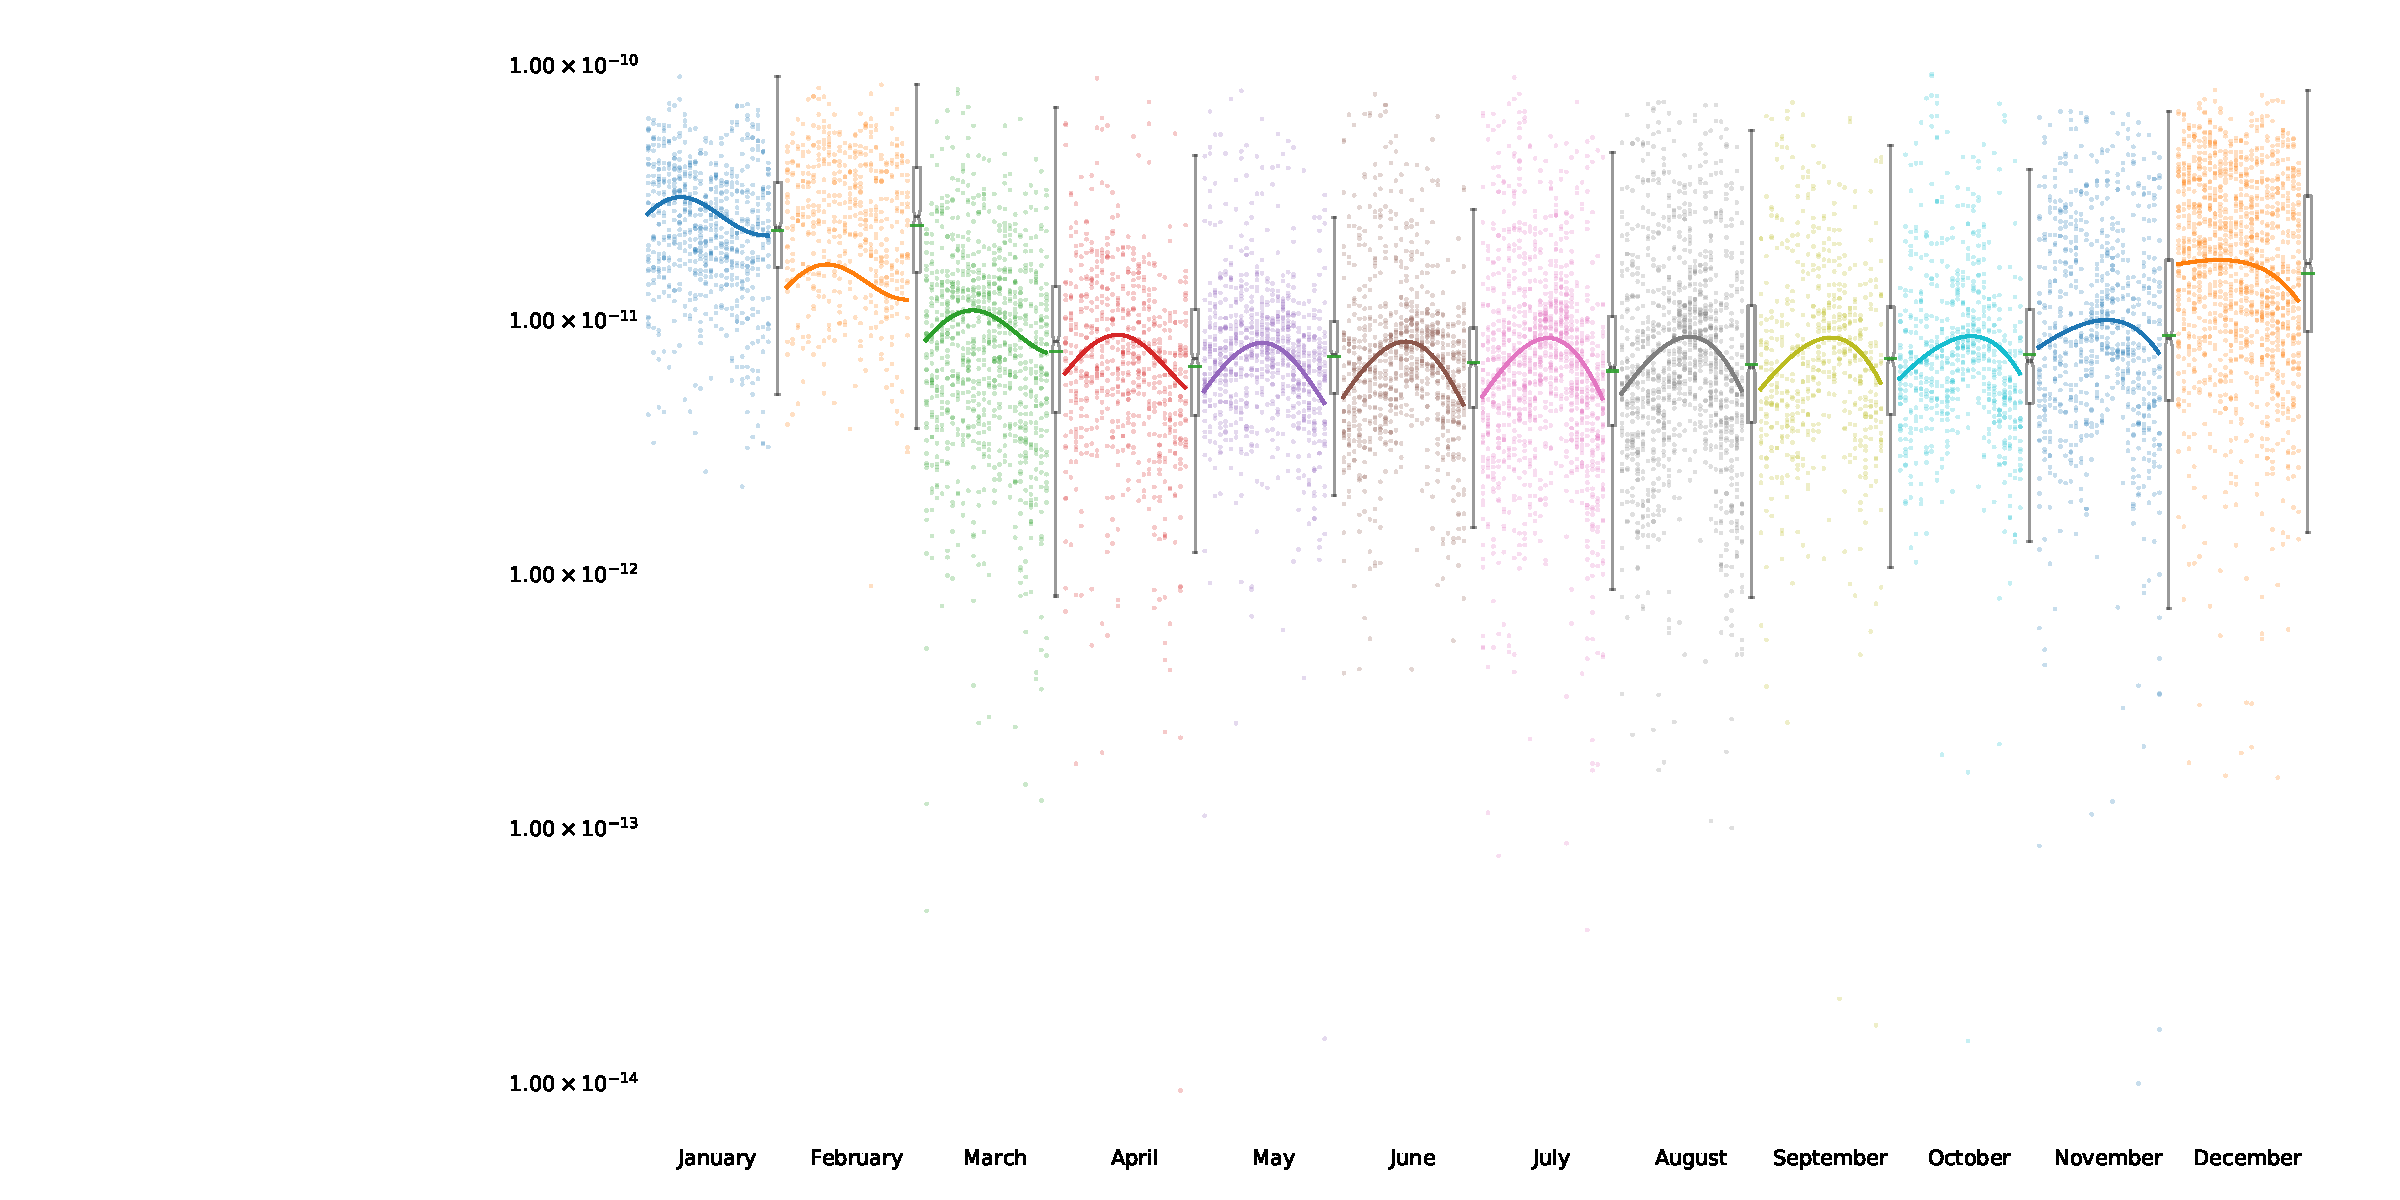
\includegraphics[width=\textwidth]{figures_c1/arc/NO2.png}
         \caption{\ce{NO2}}
         \label{fig:no2}
     \end{subfigure}
     \begin{subfigure}[b]{.4\textwidth}
         \centering
         \includegraphics[width=\textwidth]{figures_c1/arc/KBPAN.png}
         \caption{MCM reactions at the KBPAN rate.}
         \label{fig:kbpan}
     \end{subfigure}
      \caption{\textbf{ Arc diagram features for the PAN reactions. } }
        \label{fig:panno2}
\end{figure}



%
%


\subsubsection{The Traditional Network Graph}\label{sec:tradnetconc}

Finally, we have the traditional network representation in the form of a mathematical graph. Here species are represented as nodes (circles) and reactions as the links (lines) between them. This analogy has its roots in social representation and can be described using the metaphor of people holding hands - a concept familiar to most people. Graph representations allow for an overview of the structural relationships within the MCM network, and even to compare it against other reduced mechanisms, \autoref{fig:graphc1}
Here two 





 shows the comparison of the MCM against the reduced Common Representative Intermediates (CRI) \citep{cri} mechanism. In fixing common species (generally the primary emitted VOCs) between both mechanisms, we can use the graph as a fingerprint to compare changes in network structure. The CRI mechanism reduces the number of species within the MCM based on their ozone-forming potential. This is seen within the enclosed polygons in \autoref{fig:graphc1}, where the messy structure of the MCM (top) is greatly reduced, forming clusters of lumped species with similar ozone-forming potential (bottom). This form of representation is the most intuitive and commonly used sociograph, and therefore shall further be explored in \autoref{ch2}.



\begin{figure}[H]
     \centering
         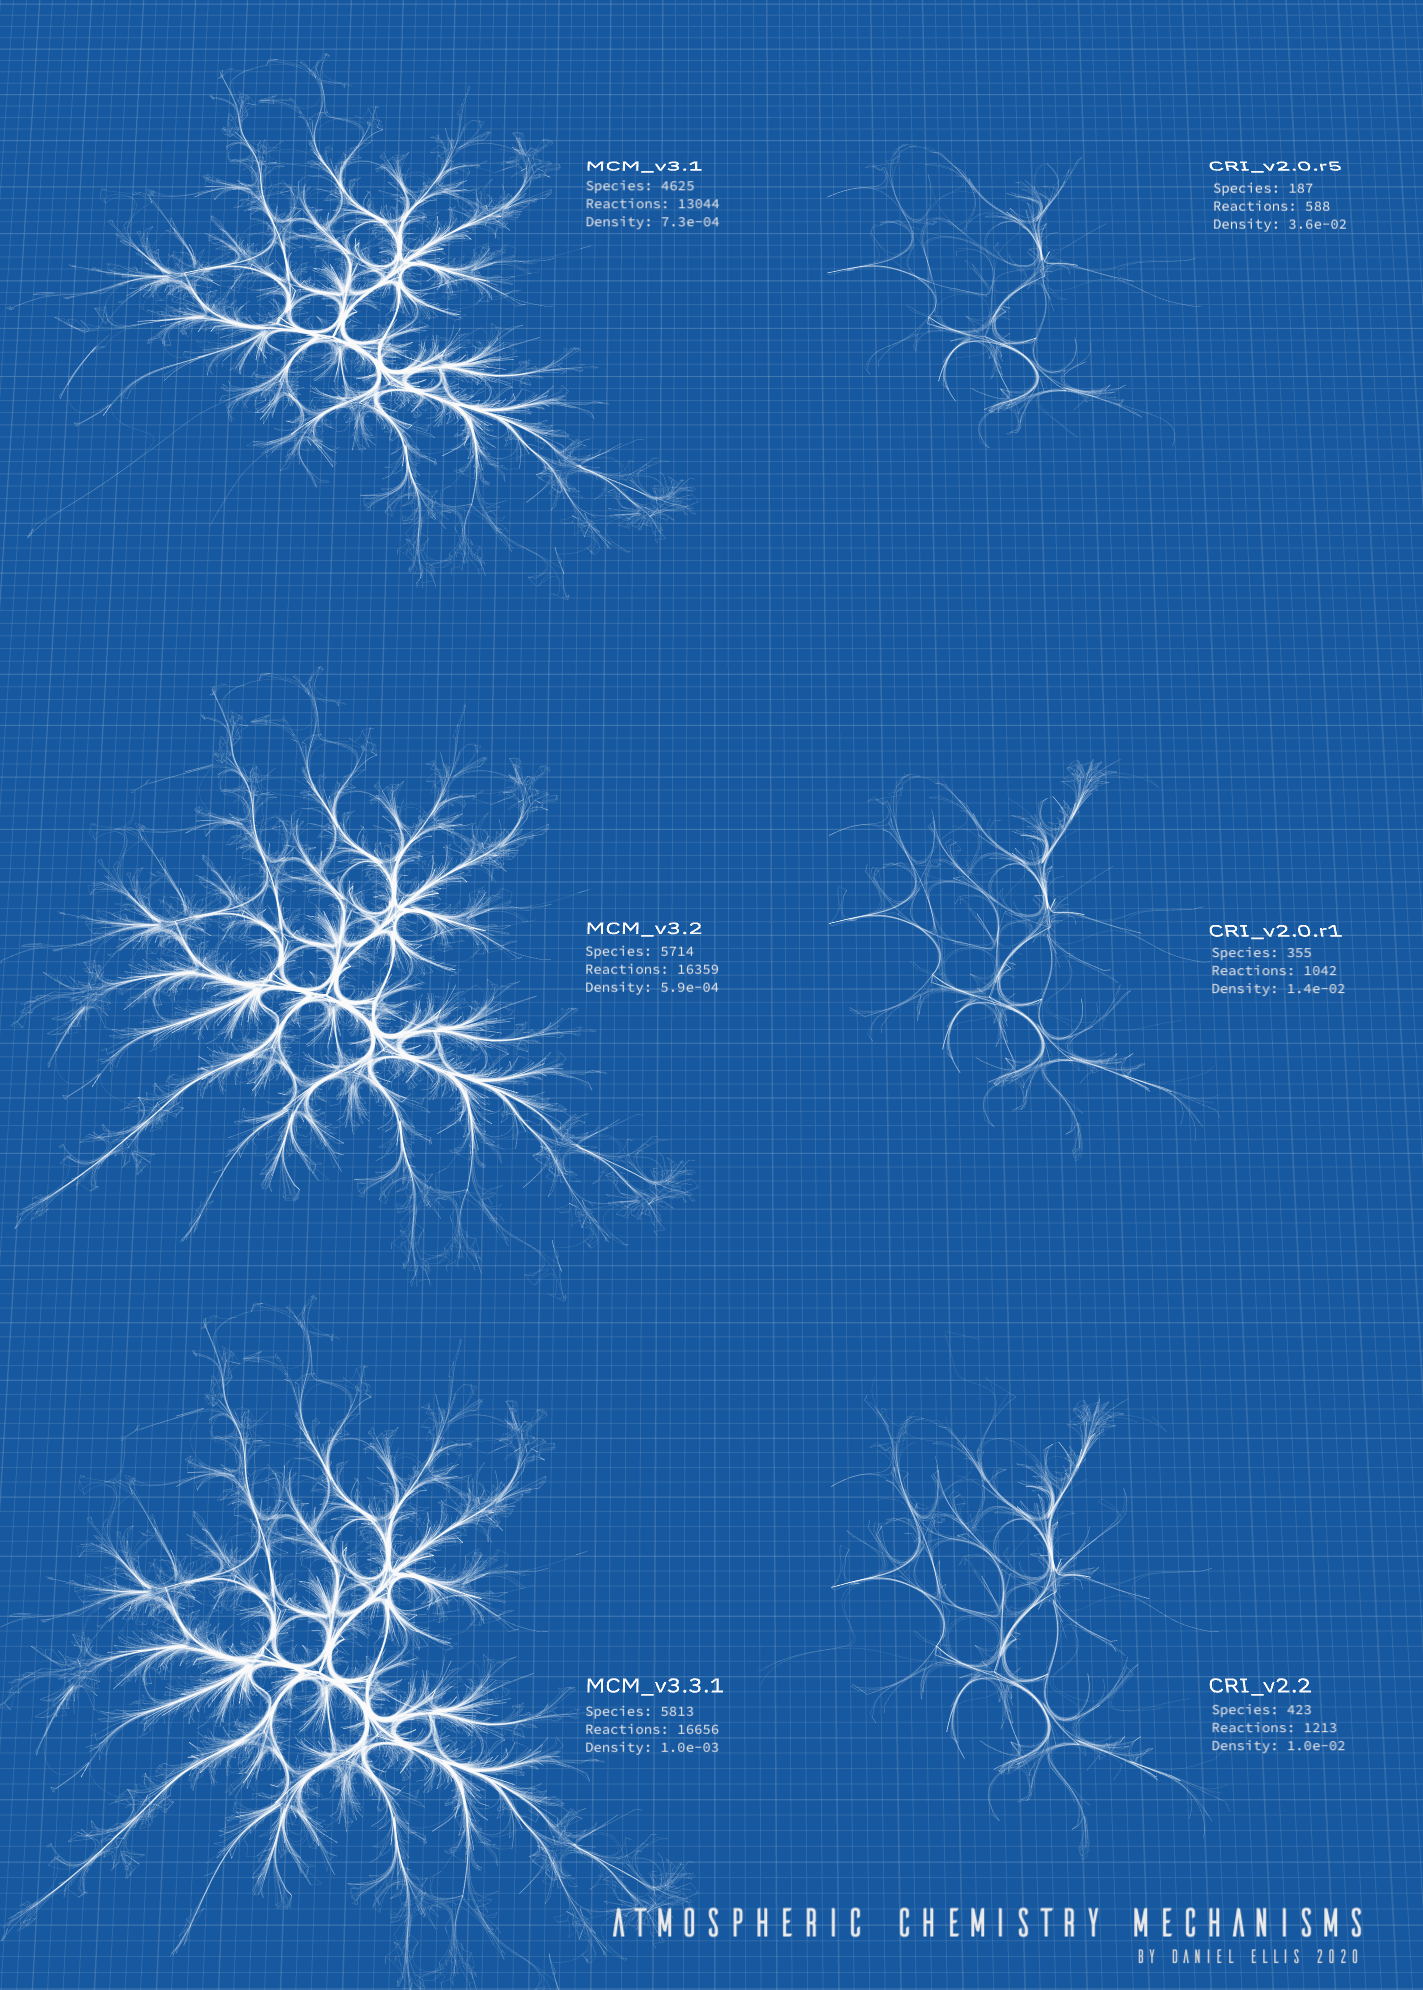
\includegraphics[width=1.1\textwidth]{poster.png}
        \caption{\textbf{Comparing a range of MCM and CRI mechanims using their graph shape and structure.} }
        \label{fig:graphc1}
\end{figure}

%
%



\section{Conclusion}

Human cognitive capacity is limited in its skill to comprehend complex information. The use of visualisation can alleviate some of this difficulty by employing our inherent pattern recognition ability and exporting the problem to exist outside our brains. Using storytelling and narrative can not only help us understand a problem but also enables us to explain it to other people. This is particularly important when trying to convey an essential subject to a non-expert audience, such as policymakers or the public.

If the data is relational, a node-link style sociograph provides the best visual representation of the data. We have explored several different sociographs (chord, arc and graph) and found that the graph format provides the most straightforward and most practical approach for the representation of the MCM chemical mechanism. This approach appears to highlight the features of the network structure while allowing us to compare and contrast different atmospheric chemical mechanisms. It is for this reason that \autoref{ch2} will further explore the use of graph-based representation in representing different chemical schemes of the atmosphere.
